%\documentclass[sigplan,nonacm]{acmart}\settopmatter{printfolios=true,printccs=false,printacmref=false}

%% For double-blind review submission, w/o CCS and ACM Reference (max submission space)
%\documentclass[acmsmall,review,anonymous]{acmart}\settopmatter{printfolios=true,printccs=false,printacmref=false}
\documentclass[acmsmall,review]{acmart}\settopmatter{printfolios=true,printccs=false,printacmref=false}
%% For double-blind review submission, w/ CCS and ACM Reference
%\documentclass[sigplan,review,anonymous]{acmart}\settopmatter{printfolios=true}
%% For single-blind review submission, w/o CCS and ACM Reference (max submission space)
%\documentclass[sigplan,review]{acmart}\settopmatter{printfolios=true,printccs=false,printacmref=false}
%% For single-blind review submission, w/ CCS and ACM Reference
%\documentclass[sigplan,review]{acmart}\settopmatter{printfolios=true}
%% For final camera-ready submission, w/ required CCS and ACM Reference
%\documentclass[acmsmall]{acmart}\settopmatter{}

%% Journal information
%% Supplied to authors by publisher for camera-ready submission;
%% use defaults for review submission.
\acmJournal{PACMPL}
\acmVolume{1}
\acmNumber{CONF} % CONF = POPL or ICFP or OOPSLA
\acmArticle{1}
\acmYear{2019}
\acmMonth{1}
\acmDOI{} % \acmDOI{10.1145/nnnnnnn.nnnnnnn}
\startPage{1}

%% Copyright information
%% Supplied to authors (based on authors' rights management selection;
%% see authors.acm.org) by publisher for camera-ready submission;
%% use 'none' for review submission.
\setcopyright{none}
%\setcopyright{acmcopyright}
%\setcopyright{acmlicensed}
%\setcopyright{rightsretained}
%\copyrightyear{2018}           %% If different from \acmYear

%% Bibliography style
\bibliographystyle{ACM-Reference-Format}
%% Citation style
\citestyle{acmauthoryear}  %% For author/year citations
%\citestyle{acmnumeric}     %% For numeric citations
%\setcitestyle{nosort}      %% With 'acmnumeric', to disable automatic
                            %% sorting of references within a single citation;
                            %% e.g., \cite{Smith99,Carpenter05,Baker12}
                            %% rendered as [14,5,2] rather than [2,5,14].
%\setcitesyle{nocompress}   %% With 'acmnumeric', to disable automatic
                            %% compression of sequential references within a
                            %% single citation;
                            %% e.g., \cite{Baker12,Baker14,Baker16}
                            %% rendered as [2,3,4] rather than [2-4].


%%%%%%%%%%%%%%%%%%%%%%%%%%%%%%%%%%%%%%%%%%%%%%%%%%%%%%%%%%%%%%%%%%%%%%
%% Note: Authors migrating a paper from traditional SIGPLAN
%% proceedings format to PACMPL format must update the
%% '\documentclass' and topmatter commands above; see
%% 'acmart-pacmpl-template.tex'.
%%%%%%%%%%%%%%%%%%%%%%%%%%%%%%%%%%%%%%%%%%%%%%%%%%%%%%%%%%%%%%%%%%%%%%


%% Some recommended packages.
\usepackage{booktabs}   %% For formal tables:
                        %% http://ctan.org/pkg/booktabs
\usepackage{subcaption} %% For complex figures with subfigures/subcaptions
                        %% http://ctan.org/pkg/subcaption

\usepackage[utf8]{inputenc}
\usepackage[T1]{fontenc}
\usepackage[scaled=0.83]{beramono}
\usepackage{amsmath}
\usepackage{amssymb}
%\usepackage{MnSymbol}
\usepackage{color}
\usepackage{xcolor,colortbl}
\usepackage{url}
\usepackage{listings}
\usepackage{paralist}
%\usepackage[compact]{titlesec}
\usepackage[font={small}]{caption}
\usepackage{wrapfig}
\usepackage{enumitem}
\usepackage{multicol}
\usepackage{flushend}
\usepackage{bcprules}

\usepackage{tikz}
\usetikzlibrary{matrix}

\definecolor{light-gray}{gray}{0.85}

% ----- listings

\definecolor{ckeyword}{HTML}{7F0055}
\definecolor{ccomment}{HTML}{3F7F5F}
\definecolor{cstring}{HTML}{2A0099}

\lstdefinelanguage{Scala}%
{morekeywords={abstract,%
  case,catch,char,class,%
  def,do,else,extends,final,finally,for,%
  if,import,implicit,%
  match,module,%
  new,null,undefined,%
  fun,array,
  override,%
  package,private,protected,public,%
  for,public,return,super,%
  this,throw,trait,try,type,%
  val,var,%
  with,while,%
  let,skip,assert,then,fst,snd,root,idx,sum,prod,exists,forall,%
  yield%
  },%
  sensitive,%
  moredelim=*[il][\bfseries]{\#\#\ },
  morecomment=[l]//,%
  morecomment=[s]{/*}{*/},%
  morestring=[b]",%
%  morestring=[b]',%
  showstringspaces=false%
}[keywords,comments,strings]%

\lstset{language=Scala,%
  mathescape=true,%
%  columns=[c]fixed,%
%  basewidth={0.5em, 0.40em},%
  aboveskip=2pt,%\smallskipamount,
  belowskip=1pt,%\negsmallskipamount,
  lineskip=-3pt,
  basewidth={0.58em, 0.45em},%
%  backgroundcolor=\color{listingbg},
  basicstyle=\footnotesize\ttfamily,
  keywordstyle=\keywordstyle,
  commentstyle=\commentstyle,
  stringstyle=\stringstyle,
%  xleftmargin=0.5cm
  literate={-->}{{$\to$}}3 
           {->}{{$\mapsto$}}3 
           {=>}{{$\Rightarrow ~$}}2 
           {|-}{{$\ts$}}2 
           %{fun}{{$\lambda$}}1 
           {idx}{{$\#$}}1 
           {sum}{{$\Sigma$}}1 
           {array(}{{$\langle.\rangle$(}}3 
           %{[[}{{$[\![$}}1
           %{]]}{{$]\!]$}}1
           %{…}{{$\!...$}}1 
}

\definecolor{listingbg}{RGB}{240, 240, 240}

\newcommand{\commentstyle}[1]{\color{ccomment}\itshape{#1}}
\newcommand{\keywordstyle}[1]{\color{ckeyword}\bfseries{#1}}
\newcommand{\stringstyle}[1]{\color{cstring}\bfseries{#1}}

\lstnewenvironment{listing}{\lstset{language=Scala}}{}
\lstnewenvironment{listingtiny}{\lstset{language=Scala,basicstyle=\scriptsize\ttfamily}}{}

\newcommand{\code}[1]{\lstinline[language=Scala,columns=fixed,basicstyle=\ttfamily]|#1|}


\newcommand{\IMP}[0]{\texttt{IMP}}
\newcommand{\FUN}[0]{\texttt{FUN}}

\newcommand{\TOOL}[0]{\texttt{SIGMA}}



% ----- packed items, so we don't waste space
\newenvironment{sitemize}{
\begin{itemize}[leftmargin=2.5ex]
  \setlength{\itemsep}{1pt}
  \setlength{\parskip}{0pt}
  \setlength{\parsep}{0pt}
}{\end{itemize}}

\newenvironment{senumerate}{
\begin{enumerate}[leftmargin=2.5ex]
  \setlength{\itemsep}{1pt}
  \setlength{\parskip}{0pt}
  \setlength{\parsep}{0pt}
}{\end{enumerate}}

\newcommand{\mypar}[1]{{\bf #1.}}

% ----- formal

%\newcommand{\judgement}[2]{{\bf #1} \hfill #2}
%\newcommand{\den}[1]{$\left\llbracket$\;#1\;$\right\rrbracket$}
\newcommand{\den}[1]{\llbracket~#1~\rrbracket}

%\newcommand{\ts}{\,\vdash\,}
\newcommand{\evalsto}{\Downarrow}

\newcommand{\mbind}{\;{\small{\texttt{>>}\hspace{-0.3pt}\raisebox{-0.15pt}{\texttt{=}}}}\;}

%\newcommand{\mbind}{{\small{\texttt{>>}\hspace{-1.7pt}\raisebox{-0.15pt}{\texttt{=}}}}}

\newcommand{\rref}[1]{\textsc{(#1)}}

% ----- comments and todo

\newcommand{\note}[1]{{\color{red}[#1]}}
\newcommand{\todo}[1]{\note{TODO: #1}}

\newcommand{\silent}[1]{}



\newcommand{\updownarrows}{\mathbin\uparrow\hspace{-.5em}\downarrow}
\newcommand{\downuparrows}{\mathbin\downarrow\hspace{-.5em}\uparrow}

\begin{document}

%% Title information
%\title{Staged Abstract Interpreters}         %% [Short Title] is optional;
\title{Staged Abstract Interpreters}         %% [Short Title] is optional;
                                        %% when present, will be used in
                                        %% header instead of Full Title.
%\titlenote{with title note}             %% \titlenote is optional;
                                        %% can be repeated if necessary;
                                        %% contents suppressed with 'anonymous'
%\subtitle{Fast and Compositional Whole-Program Analysis for Free}                     %% \subtitle is optional
\subtitle{Fast and Modular Whole-Program Analysis via Meta-Programming}                     %% \subtitle is optional
%\subtitlenote{with subtitle note}       %% \subtitlenote is optional;
                                        %% can be repeated if necessary;
                                        %% contents suppressed with 'anonymous'

\iffalse
\author
[Guannan Wei, Yuxuan Chen, Tiark Rompf]
{
\vspace{-2ex}
Guannan Wei, Yuxuan Chen, Tiark Rompf\\
Purdue University
\vspace{-0.5ex}
}
\fi


%% Author information
%% Contents and number of authors suppressed with 'anonymous'.
%% Each author should be introduced by \author, followed by
%% \authornote (optional), \orcid (optional), \affiliation, and
%% \email.
%% An author may have multiple affiliations and/or emails; repeat the
%% appropriate command.
%% Many elements are not rendered, but should be provided for metadata
%% extraction tools.

%% Author with single affiliation.
\author{Guannan Wei}
\author{Yuxuan Chen}
\author{Tiark Rompf}
%\authornote{with author1 note}          %% \authornote is optional;
                                        %% can be repeated if necessary
%\orcid{nnnn-nnnn-nnnn-nnnn}             %% \orcid is optional
\affiliation{
  %\position{Position1}
  \department{Department of Computer Science}              %% \department is recommended
  \institution{Purdue University}            %% \institution is required
  %\streetaddress{305 N. University Street}
  %\city{West Lafayette}
  %\state{IN}
  %\postcode{47906}
  \country{USA}                    %% \country is recommended
}
\email{guannanwei@purdue.edu}          %% \email is recommended
\email{chen1797@purdue.edu}
\email{tiark@purdue.edu}          %% \email is recommended

%% Author with two affiliations and emails.
%\authornote{with author2 note}          %% \authornote is optional;
                                        %% can be repeated if necessary
%\authornote{with author1 note}          %% \authornote is optional;
                                        %% can be repeated if necessary
%\orcid{nnnn-nnnn-nnnn-nnnn}             %% \orcid is optional

\lstMakeShortInline[keywordstyle=,%
                    flexiblecolumns=false,%
                    %basewidth={0.56em, 0.52em},%
                    mathescape=false,%
                    basicstyle=\tt]@

%% Abstract
%% Note: \begin{abstract}...\end{abstract} environment must come
%% before \maketitle command
\begin{abstract}
  It is well known that a staged interpreter is a compiler: specializing an
interpreter to a given program produces an equivalent executable that runs faster.
This connection is known as the first Futamura projection.
It is even more widely known that an abstract interpreter is a program analyzer:
tweaking an interpreter to run on abstract domains produces a sound static
analysis. What happens when we combine these two ideas, and apply specialization to
an \emph{abstract} interpreter?

In this paper, we present a unifying framework that naturally extends the first
Futamura projection from concrete interpreters to abstract interpreters. Our
approach derives a sound staged abstract interpreter based on a
semantic-agnostic interpreter with type-level binding-time abstractions and
monadic abstractions. By using different instantiations of these abstractions,
the generic interpreter can flexibly behave in one of four modes: as an unstaged
concrete interpreter, a staged concrete interpreter, an unstaged abstract
interpreter, or a staged abstract interpreter. As an example of
\emph{abstraction without regret}, the overhead of these abstraction layers is
eliminated in the generated code after staging. We show that staging abstract
interpreters is practical and useful to optimize static analysis, all while
requiring less engineering effort and without compromising soundness. We conduct
three case studies, including a comparison with Boucher and Feeley's abstract
compilation, applications to various control-flow analyses, and a demonstration
that can be used for modular analysis. We also empirically evaluate the effect
of staging on the execution time. The experiment shows an order of magnitude
speedup with staging for control-flow analyses.

\iffalse
We obtain a sound static analysis, specialized for
a given program, that runs faster. More surprisingly, we show that by applying
the staged abstract interpreter to \textit{open} programs and considering the
free variables as dynamic inputs, we obtain a modular analysis that generates
sound partial analysis results which can be composed and reused later without
losing precision, even though the original abstract interpreter is a
whole-program analysis algorithm.

Based on the idea of staged abstract interpreters, we show several case studies,
including \citeauthor{Boucher:1996:ACN:647473.727587}'s abstract compilation of
0-CFA, pushdown control-flow analysis with context-sensitivity and precise
stores, and a numerical analysis on an imperative language.

We empirically evaluate the performance improvements on control-flow analysis of
benchmark programs. The results show speedups up to 2.3x with staging on a
monovariant analysis.
\fi

% It is well known that a staged interpreter is a compiler, which provides
% performance improvement by specializing the interpreter to a given program. In
% this paper, we study \textit{abstract} interpreters combined with multi-stage
% programming, i.e., the staged abstract interpreters. By staging the abstract
% interpreter with respect to a program, we obtain a specialized analysis that
% runs faster. By applying the staged abstract interpreter with \textit{open}
% programs and considering the free variables as dynamic inputs, we obtain a
% modular analysis that generates sound partial analysis results which can be
% composed and reused later without losing precision, though the original
% abstract interpreter is a whole-program analysis algorithm. Using the idea of
% staged abstract interpreters, we show several case studies, including
% \citeauthor{Boucher:1996:ACN:647473.727587}'s abstract compilation of 0-CFA,
% pushdown control-flow analysis with context/path/flow-sensitivity and
% store-widening, and a numerical analysis on an imperative language. We also
% empirically evaluate the improvement of performance on control-flow analysis
% of benchmark programs. The result shows an average speedup of Nx when staging
% to Scala for a monovariant analysis, and Mx for polyvariant analysis.

\end{abstract}


%% 2012 ACM Computing Classification System (CSS) concepts
%% Generate at 'http://dl.acm.org/ccs/ccs.cfm'.
\begin{CCSXML}
<ccs2012>
<concept>
<concept_id>10011007.10011006.10011008</concept_id>
<concept_desc>Software and its engineering~General programming languages</concept_desc>
<concept_significance>500</concept_significance>
</concept>
<concept>
<concept_id>10003456.10003457.10003521.10003525</concept_id>
<concept_desc>Social and professional topics~History of programming languages</concept_desc>
<concept_significance>300</concept_significance>
</concept>
</ccs2012>
\end{CCSXML}

\ccsdesc[500]{Software and its engineering~General programming languages}
\ccsdesc[300]{Social and professional topics~History of programming languages}
%% End of generated code


%% Keywords
%% comma separated list
% \keywords{keyword1, keyword2, keyword3}  %% \keywords are mandatory in final camera-ready submission


%% \maketitle
%% Note: \maketitle command must come after title commands, author
%% commands, abstract environment, Computing Classification System
%% environment and commands, and keywords command.
\maketitle

\iffalse

\renewcommand\thefootnotecopyrightpermission{}
\footnotetextcopyrightpermission{
Preprint, November 2018.\\ Copyright held by the authors.}
\fancyhead[RO,LE]{Preprint, November 2018}

\fi

\section{Introduction} \label{intro}

Abstract interpretation as a lattice-based approach to sound static analyses was
proposed by \citet{DBLP:conf/popl/CousotC77, CousotCousot79-1}. Based on the notion of Galois
connections, the analyzer can soundly approximate the
concrete program behavior at runtime by computing fixed points on an abstract
domain. Despite the tremendous theoretical development of abstract
interpretation over the years, constructing artifacts and analyzers that perform
sound abstract interpretation for modern and expressive languages was considered
complicated for a long time.

Recent progress on methodologies such as Abstracting Abstract Machine (AAM)
\cite{DBLP:journals/jfp/HornM12, DBLP:conf/icfp/HornM10} uncovers an
operational approach to constructing abstract interpreters.  By deriving
semantics artifacts for abstract interpretation from their concrete
counterparts (for example, abstract machines), soundness can be easily
established by examining the transformation of semantic artifacts.
This systematic abstraction approach can be tailored to different
language features (such as state, first-class control, exceptions, and
concurrency) and sensitivity analyses \cite{DBLP:conf/icfp/Gilray0M16,
  DBLP:conf/popl/GilrayL0MH16, Darais:2015:GTM:2814270.2814308}. It
has also been applied to various small-step abstract machines
\cite{DBLP:journals/jfp/HornM12, DBLP:conf/icfp/HornM10,
  Sergey:2013:MAI:2491956.2491979} and big-step definitional
interpreters \cite{Wei:2018:RAA:3243631.3236800,
  DBLP:journals/pacmpl/DaraisLNH17, Keidel:2018:CSP:3243631.3236767}.

%Based on the idea of abstracting abstract machines, more
%pragmatically, several implementation strategies utilizing purely
%functional programming techniques to build abstract interpreters have
%emerged. 

Based on the idea of AAM, more pragmatically, several implementation strategies
in high-level functional programming languages have emerged.  Such techniques
include monads and monad transformers \cite{DBLP:journals/pacmpl/DaraisLNH17,
Sergey:2013:MAI:2491956.2491979}, arrows
\cite{Keidel:2018:CSP:3243631.3236767}, extensible effects
\cite{Kiselyov:2015:FMM:2804302.2804319, Githubsemantic}, etc. These pure
approaches provide certain benefits, for example, the abstract interpretation
artifacts can be built in a compositional and modular fashion, and referential
transparency allows programmers to confidently reason about the correctness of
their implementations.  The soundness of an analysis can also be proven with less
effort, whether by mechanized proofs \cite{Darais:2016:CGC:2951913.2951934} or
paper-based proofs \cite{Keidel:2018:CSP:3243631.3236767}.  

However, besides the intrinsic complexity of static analysis, there are
additional abstraction penalties from these high-level implementation
approaches. First, similar to concrete interpreters, an abstract interpreter
analyzes a program by traversing its AST. This traversal incurs
interpretive overhead, such as pattern matching on the AST nodes and recursive
calls on subexpressions. If it is a single-time traversal, such overhead can be
negligible. But usually, abstract interpreters iteratively analyze and traverse
the AST multiple times to reach fixed-points, therefore the accumulated
overhead is even magnified. 
%Repeatedly analyzing library programs also poses significant overhead.
%Such overhead can be negligible if the abstract
%interpreter only runs on the program a single time, but can accumulate
%significantly if it runs repeatedly (for example, on libraries).  
Second, it is common that abstract interpreters written in pure languages
extensively use functional encodings of side-effects to implement the semantics
of abstract interpretation.  For example, the list monad can be used to model
nondeterminism from collecting interpreters.
Although such pure approaches have their own merits, compared with imperative,
stateful implementations, they are significantly slower.  In order to
reconcile these approaches, one must use a programming technique which allows
for high-level abstractions during implementation, but bypasses the
incurred overhead at runtime.

Roughly at the same time when abstract interpretation was proposed in the
1970s, \citet{futamura1971partial} observed a close
connection between interpreters and compilers through a hierarchy of
specializations, since then known as Futamura Projections. The first Futamura
projection describes that specializing an interpreter to the input program
removes interpretative overhead and yields an equivalent executable
that runs faster. 
In recent years, the idea of Futamura projections has regained more attentions
and successfully applied to many real-world problems, examples including
query compilers \cite{DBLP:conf/sigmod/TahboubER18}, PyPy \cite{Bolz:2009:TMP:1565824.1565827},
Truffle \cite{Marr:2015:TVP:2814270.2814275}, etc.
The challenge here: can we apply the same idea to a general abstract interpreter
to make it run faster? The solution is not obvious, as we need to specialize
a nonstandard semantics that extensively uses nondeterminism, operates on
abstract domains, and computes fixed-points iteratively over a cache. 

In this paper, we show that the first Futamura projection can be naturally
extended to abstract interpreters. We present an abstraction-without-regret
framework that eliminates performance penalties for monadic abstract
interpreters, while keeping the implementation as close to their conceptual
model as possible.
In short, our approach borrows ideas and techniques from multi-stage
programming and embedded DSLs, and apply them to abstract interpreters:  1) To
remove the overhead from interpretation and effect layers, we specialize the
abstract interpreter via staging and then generate efficient low-level code
that does the actual analysis. 2) Inspired by the tagless-final interpreters
\cite{DBLP:journals/jfp/CaretteKS09}, we construct a generic interpreter that
abstracts over binding-times and different semantics, which allows the staged
abstract interpreter to be derived from its unstaged counterpart.  As a result,
the derived staged abstract interpreters has no intrusive changes to the
underlying abstract semantics, thereby preserving soundness.  In this
sense, our approach allows for no regret for both performance and engineering
effort. We elaborate these two main ideas in detail, as follows.

%The result of specialization is reusable, and the effect layers have
%been eliminated in the generated code.

\vspace{-1em}
\begin{figure}[h]
  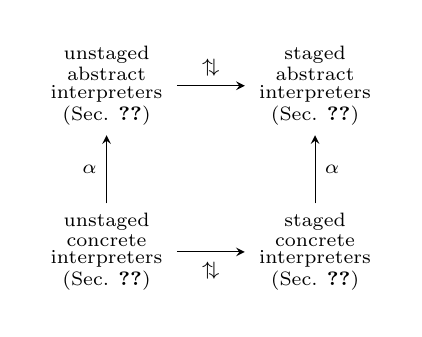
\begin{tikzpicture}
  \matrix (m) [matrix of math nodes,row sep=2.5em,column sep=2.5em,minimum width=2em]
  {
    \begin{smallmatrix} \text{unstaged} \\ \text{abstract} \\ \text{interpreters} \\ (\text{Sec.}~\ref{unstaged_abs}) \end{smallmatrix} &
    \begin{smallmatrix} \text{staged} \\ \text{abstract} \\ \text{interpreters} \\ (\text{Sec.}~\ref{sai}) \end{smallmatrix} \\
    \begin{smallmatrix} \text{unstaged} \\ \text{concrete} \\ \text{interpreters} \\ (\text{Sec.}~\ref{unstaged_conc}) \end{smallmatrix} &
    \begin{smallmatrix} \text{staged} \\ \text{concrete} \\ \text{interpreters} \\ (\text{Sec.}~\ref{stagedinterp}) \end{smallmatrix} \\ };
  \path[-stealth]
    (m-1-1) edge node [above, font=\scriptsize] {$\updownarrows$} (m-1-2)
    (m-2-1) edge node [left, font=\scriptsize] {$\alpha$} (m-1-1)
    (m-2-1) edge node [below, font=\scriptsize] {$\updownarrows$} (m-2-2)
    (m-2-2) edge node [right, font=\scriptsize] {$\alpha$} (m-1-2);
  \end{tikzpicture}
  \vspace{-0.5em}
  \caption{The confluence of specialization and approximation.}
  \label{confluence}
\end{figure}
\vspace{-1em}


\paragraph{Futamura Projection of Abstract Interpreters}

The first Futamura projection specifically shows that specializing an
interpreter w.r.t. the input program yields an equivalent executable. For
instance, assume that @eval : Expr --> Input --> Value@ is an interpreter for some language.
Given a program $e_0$@ : Expr@, by applying the specialization, we can
obtain a specialized program $\texttt{eval}_{\texttt{e0}}$ : @Input --> Value@.
%which is the so-called \textit{equivalent executable}.
% By definition of the interpreter, they produce the same result when applied with the argument $\texttt{eval}_{\texttt{e0}}(arg) = [\![ e_0 ]\!] arg $.
The first proposed approach to realize Futamura projections is partial
evaluation \cite{DBLP:books/daglib/0072559}, which relies on an automatic
binding-time analysis (\textit{static} or \textit{dynamic}).  The underlying
representation can be viewed as a \textit{two-level semantics}
\cite{NIELSON1989117, NIELSON198859} that distinguishes compile-time
computation and run-time computation.
However, it is hard to precisely analyze binding-times given an arbitrary
program. As an alternative approach, multi-stage programming (MSP)
\cite{taha1999multi, DBLP:conf/pepm/TahaS97} allows users to explicitly program over
a two-level syntax \cite{Nielson:1992:TFL:130665}, by manually
annotating the binding-times of variables. Then, the MSP system
will check whether these annotations are consistent, and specialize the program
using that information. The staging annotations can be either syntactic (e.g.,
quote and quasi-quote in MetaML/MetaOCaml) or type-based (e.g., the Lightweight
Modular Staging framework \cite{DBLP:conf/gpce/RompfO10} in Scala).

To apply Futamura projections on abstract interpreters, we consider
\citet{DBLP:journals/pacmpl/DaraisLNH17}'s big-step monadic abstract
interpreter as the unstaged baseline.  Similar to the two-level semantics
\cite{NIELSON1989117}, monads provide a good abstraction to hide the detail of
abstract interpretation semantics. However, monads do not have a clear
stage distinction.
We further introduce binding-times and make the monads binding-time polymorphic.
Our proposed framework adopts the type-based multi-stage programming from the
Lightweight Modular Staging framework, and implements the Futamura projection
of an abstract interpreter for a stateful higher-order
language. By deriving staged monads that can be used to perform code generation, we
obtain a staged abstract interpreter that can be used for specialization. Through
staging, the generated code is specialized to the input program, and all the
monadic operations are inlined and compiled down to low-level Scala code.

\paragraph{Generic Interpreter and Reinterpretation}

Program specialization and abstract interpretation are two orthogonal
concepts.  To implement the confluence of them, we first construct a
generic interpreter that is agnostic to both binding times and value
domains used in the semantics.  Later, the generic interpreter can be
instantiated from these two dimensions (Figure~\ref{confluence}):
\begin{itemize}
\item With a flat binding-time and concrete domains, it is an ordinary
  definitional interpreter based on big-step operational semantics;
\item With two-level binding-times and concrete domains, it is a
  compiler that translates a program into another language;
\item With a flat binding-time and abstract domains, it is a
  definitional abstract interpreter \cite{DBLP:journals/pacmpl/DaraisLNH17}
  that statically computes runtime properties;
\item With two-level binding-times and abstract domains, it is an optimizing
  program analyzer, but works in the fashion of compilation.
\end{itemize}

Although the four artifacts may look dissimilar at first glance, they in
fact are all firmly rooted in the concrete semantics of the language.  This
observation provides a way to abstract over the interpreter and achieve the
flexibility of reinterpreting the shared interpreter.  The generic interpreter
returns a value of monadic type, which can be varied by different semantics.
The value domains of the interpreter and the effects such as state and nondeterminism
can all be wrapped into this monadic type.  The binding-time abstraction is
represented by a higher-kinded type, and injected into the monadic type.  The
binding-times control whether the interpreter produces values directly or
generates code. 

%It is worth mentioning
%that the binding-time type is also injected into the monadic type, so that we
%will distinguish normal monads and staged monads.

\paragraph{Applications and Evaluation}
We evaluate the idea of staging an abstract interpreter through
case studies and an empirical performance evaluation.
1) We compare our approach with abstract compilation
\cite{Boucher:1996:ACN:647473.727587}, an implementation technique for
control-flow analyses. We show that by utilizing type-based stage
annotations, we can achieve the same optimizations. Meanwhile,
the analyzer does not need to change, except the addition of stage annotations,
thereby requiring significantly less engineering effort.
2) We extend the basic staged abstract interpreter to different flow
analyses, including a store-widened analysis, a context-sensitive
analysis, and abstract garbage collection.
3) We show that staging an abstract interpreter enables modular
compilation of an analysis to programs. Here we borrow the concept of
modular analysis, and show that the compiled analysis is reusable.
Therefore, the approach provides a modular way to create optimized
analysis code by mechanized reuse of a whole-program analyzer.
4) We empirically evaluate the performance improvements gained by staging,
showing an order of magnitude speedup.

\paragraph{Contributions} Briefly, the contributions of the paper are as follows:
\begin{itemize}[leftmargin=2em]
  \item Intellectually, we present a framework that naturally extends the first
    Futamura projection to definitional abstract interpreters, showing a
    well-grounded approach to optimizing static analyses via meta-programming.
  \item Practically, we show that staging an abstract interpreter is useful to
    improve performance and scalability of analyses by case studies and an
    empirical evaluation.
\end{itemize}

\paragraph{Organization} The paper is organized as follows:
\begin{itemize}[leftmargin=2em]
  \item We begin by introducing our target language and reviewing
    monads in Scala, and then presenting the generic interpreter
    (Section~\ref{prelim}), after which we review instantiations
    of concrete interpretation (Section~\ref{unstaged_conc}) and
    staged concrete interpretation (Section~\ref{stagedinterp}).
  \item We present the unstaged abstract interpreter under the same
    framework by replacing the environment, store, and values to their
    abstract counterparts (Section~\ref{unstaged_abs}). We then
    show that the combination of approximation and specialization, dubbed
    \textit{staged abstract interpreters}, can be readily derived
    (Section~\ref{sai}). We also summarize the approach and discuss
    soundness properties after showing the four artifacts.
  \item We summarize our approach and discuss correctness (Section~\ref{discussion}).
    We conduct three case studies (Section~\ref{cases_study}) and
    an empirical evaluation on performance improvements (Section~\ref{evaluation}).
    Finally we discuss related work and conclude.
\end{itemize}

\iffalse
On the other side, static analysis is a trade-off between performance and
precision: higher precision usually leads to longer running time.

4. Existing method to improve the performance is adhoc, engineering heavy, require to rewrite the optimized version, therefore harder to reason about the correctness
6. program analyzers are also meta-programs, they manipulate other programs as data objects
\fi

\newcommand{\TLang}{$L_\lambda$}

\section{Preliminaries} \label{prelim}

In this section, we first describe the abstract syntax of the language for our interpreters. 
Then present the generic interpreter shared among the four different
semantics, after which, we instantiate the interpreter to the concrete one.
It is worth noting that we choose to use Scala and monadic style to
demonstrate the idea, but the approach is not restricted to our
choice. One can use imperative or direct style in other MSP languages
(e.g., MetaOCaml \cite{DBLP:conf/gpce/CalcagnoTHL03, DBLP:conf/flops/Kiselyov14}
and Template Haskell \cite{Sheard:2002:TMH:636517.636528} to construct
such staged abstract interpreters.

\subsection{Abstract Syntax} \label{bg_lang}

We consider a call-by-value $\lambda$-calculus in direct-style, extended
with numbers, arithmetic, recursions, and conditionals. Other effectful features
such as assignments can also be supported readily.
%In Section~\ref{cases_imp}, we will add more imperative features to the language.
Since we are mostly interested in analyzing the dynamic behaviors of the
program, we disguise any static semantics and type system. We also assume that
input programs are well-typed and all variables are distinct. The abstract
syntax is shown as follows:

\begin{lstlisting}
  abstract class Expr
  case class Lit(i: Int) extends Expr                         // numbers
  case class Var(x: String) extends Expr                      // variables
  case class Lam(x: String, e: Expr) extends Expr             // abstractions
  case class App(e1: Expr, e2: Expr) extends Expr             // applications
  case class If0(e1: Expr, e2: Expr, e3: Expr) extends Expr   // conditionals
  case class Rec(x: String, rhs: Expr, e: Expr) extends Expr  // recursions
  case class Aop(op: String, e1: Expr, e2: Expr) extends Expr // arithmetic
\end{lstlisting}

The abstract syntax we present in fact can be seen as a deep embedding of the
language -- we use data-types to represent programs. This design choice allows us
to easily use different interpretations over the AST; with the inheritance and
overriding mechanism in Scala, we may also add new language constructs and reuse
existing interpretations.

%\todo{cite Bruno?}.

\iffalse
We will give the concrete semantics using a big-step definitional
interpreter. The interpreter is a recursive function that takes the program AST,
environment, and store, and returns the evaluated value and the accompanying
store. The environment is a mapping from identifiers to addresses, and the store
is a mapping from addresses to values. We use the store to model recursion and
mutation in concrete semantics; it is also useful for polyvariant analysis. This
environment-and-store-passing style big-step interpreter is standard and can
also be obtained by refunctionalizing \cite{DBLP:conf/ppdp/AgerBDM03,
Wei:2018:RAA:3243631.3236800} a small-step CESK machine
\cite{DBLP:conf/popl/FelleisenF87}.
\fi

\subsection{Monads in Scala} \label{monadscala}

A monad is a type constructor \lstinline[keywordstyle=,flexiblecolumns=false,mathescape=false,basicstyle=\tt]{M[_]: * -> *} with two operations, often called
\lstinline[keywordstyle=,flexiblecolumns=false,mathescape=false,basicstyle=\tt]{return} and \lstinline[keywordstyle=,flexiblecolumns=false,mathescape=false,basicstyle=\tt]{bind}. Informally, \lstinline[keywordstyle=,flexiblecolumns=false,mathescape=false,basicstyle=\tt]{return} wraps a value into the monad \lstinline[keywordstyle=,flexiblecolumns=false,mathescape=false,basicstyle=\tt]{M}, and
\lstinline[keywordstyle=,flexiblecolumns=false,mathescape=false,basicstyle=\tt]{bind} unwraps the monadic value and transforms it into a new monadic value.
Pragmatically in Scala, we define a monad type class using trait \lstinline[keywordstyle=,flexiblecolumns=false,mathescape=false,basicstyle=\tt]{Monad} (Figure
\ref{fig:monad}), where it declares the \lstinline[keywordstyle=,flexiblecolumns=false,mathescape=false,basicstyle=\tt]{pure} \footnote{We elect to use
\texttt{pure} as the name, since \texttt{return} is a keyword in Scala and
\texttt{unit} is a built-in function in LMS.} and \lstinline[keywordstyle=,flexiblecolumns=false,mathescape=false,basicstyle=\tt]{flatMap} operation. The trait
itself takes the monad type \lstinline[keywordstyle=,flexiblecolumns=false,mathescape=false,basicstyle=\tt]{M[_]} as argument, which is a higher-kinded type
that takes a type and returns a type. The method \lstinline[keywordstyle=,flexiblecolumns=false,mathescape=false,basicstyle=\tt]{pure} promotes values of type
\lstinline[keywordstyle=,flexiblecolumns=false,mathescape=false,basicstyle=\tt]{A} to values of type \lstinline[keywordstyle=,flexiblecolumns=false,mathescape=false,basicstyle=\tt]{M[A]}. The monadic \lstinline[keywordstyle=,flexiblecolumns=false,mathescape=false,basicstyle=\tt]{bind} operation is usually called
\lstinline[keywordstyle=,flexiblecolumns=false,mathescape=false,basicstyle=\tt]{flatMap} in Scala, which takes a monad-encapsulated value of type \lstinline[keywordstyle=,flexiblecolumns=false,mathescape=false,basicstyle=\tt]{M[A]}, a
function of \lstinline[keywordstyle=,flexiblecolumns=false,mathescape=false,basicstyle=\tt]{A => M[B]} and returns values of type \lstinline[keywordstyle=,flexiblecolumns=false,mathescape=false,basicstyle=\tt]{M[B]}.

\begin{figure}[h!]
  \centering
  \begin{subfigure}[b]{0.55\textwidth}
    \begin{lstlisting}
  trait Monad[M[_]] {                                  
    def pure[A](a: A): M[A]                            
    def flatMap[A,B](ma: M[A])(f: A => M[B]): M[B]     
  }                                                    
    \end{lstlisting}
    \caption{trait \texttt{Monad}} \label{fig:monad}
  \end{subfigure}
  ~
  \begin{subfigure}[b]{0.4\textwidth}
    \begin{lstlisting}
trait MonadOps[M[_], A] {
  def map[B](f: A => B): M[B]
  def flatMap[B](f: A => M[B]): M[B]
}
    \end{lstlisting}
    \caption{trait \texttt{MonadOps}} \label{fig:monadops}
  \end{subfigure}
\end{figure}

Similar to Haskell's \lstinline[keywordstyle=,flexiblecolumns=false,mathescape=false,basicstyle=\tt]{do}-notation, Scala provides special syntactic support for
monadic operations through \lstinline[keywordstyle=,flexiblecolumns=false,mathescape=false,basicstyle=\tt]{for}-comprehension.
For example, an object of \lstinline[keywordstyle=,flexiblecolumns=false,mathescape=false,basicstyle=\tt]{List[A]} is an instance of \lstinline[keywordstyle=,flexiblecolumns=false,mathescape=false,basicstyle=\tt]{List} monad, where \lstinline[keywordstyle=,flexiblecolumns=false,mathescape=false,basicstyle=\tt]{A} is the element type. 
Then to compute the Cartesian product of two lists of numbers, we can use Scala's
\lstinline[keywordstyle=,flexiblecolumns=false,mathescape=false,basicstyle=\tt]{for}-comprehension syntax.
\begin{lstlisting}
  val xs = List(1, 2); val ys = List(4, 5)
  for { x <- xs; y <- ys } yield (x, y) // List((1,4), (1,5), (2,4), (2,5))
\end{lstlisting}

The Scala compiler will translate the above \lstinline[keywordstyle=,flexiblecolumns=false,mathescape=false,basicstyle=\tt]{for}-comprehension expression into
an equivalent one using \lstinline[keywordstyle=,flexiblecolumns=false,mathescape=false,basicstyle=\tt]{flatMap} and \lstinline[keywordstyle=,flexiblecolumns=false,mathescape=false,basicstyle=\tt]{map} ~\cite{scala_spec}. The last binding
in the \lstinline[keywordstyle=,flexiblecolumns=false,mathescape=false,basicstyle=\tt]{for}-comprehension is translated into a \lstinline[keywordstyle=,flexiblecolumns=false,mathescape=false,basicstyle=\tt]{map}, where the expression of
\lstinline[keywordstyle=,flexiblecolumns=false,mathescape=false,basicstyle=\tt]{yield} becomes the body expression of that \lstinline[keywordstyle=,flexiblecolumns=false,mathescape=false,basicstyle=\tt]{map} application. The foregoing
bindings in the comprehension are all translated into calls of \lstinline[keywordstyle=,flexiblecolumns=false,mathescape=false,basicstyle=\tt]{flatMap}.
\begin{lstlisting}
  xs.flatMap { case x => ys.map { case y => (x, y) } }
\end{lstlisting}

Note that here the monadic object \lstinline[keywordstyle=,flexiblecolumns=false,mathescape=false,basicstyle=\tt]{List[_]} encapsulates the data
internally.  Therefore it only exposes the simplified version of
\lstinline[keywordstyle=,flexiblecolumns=false,mathescape=false,basicstyle=\tt]{flatMap}, where the monad \lstinline[keywordstyle=,flexiblecolumns=false,mathescape=false,basicstyle=\tt]{M[A]} is not introduced as a function
argument. The trait \lstinline[keywordstyle=,flexiblecolumns=false,mathescape=false,basicstyle=\tt]{MonadOps} (Figure \ref{fig:monadops}) defines the
simplified version of monadic operations that are necessary for
\lstinline[keywordstyle=,flexiblecolumns=false,mathescape=false,basicstyle=\tt]{for}-comprehension. The conversion between \lstinline[keywordstyle=,flexiblecolumns=false,mathescape=false,basicstyle=\tt]{Monad} and \lstinline[keywordstyle=,flexiblecolumns=false,mathescape=false,basicstyle=\tt]{MonadOps}
can be done by using the implicit design pattern.
In the rest of the paper, we use Scala's \lstinline[keywordstyle=,flexiblecolumns=false,mathescape=false,basicstyle=\tt]{for}-comprehension syntax
and a few of monads and monad transformers such as \lstinline[keywordstyle=,flexiblecolumns=false,mathescape=false,basicstyle=\tt]{ReaderT},
\lstinline[keywordstyle=,flexiblecolumns=false,mathescape=false,basicstyle=\tt]{StateT}, and \lstinline[keywordstyle=,flexiblecolumns=false,mathescape=false,basicstyle=\tt]{ListT/SetT} to write our interpreters. The implementation
of monads and monad transformers essentially borrows the ground-truth
from Haskell.

\subsection{Generic Interpreter} \label{generic_if}

Monad transformers are type constructors of kind \lstinline[keywordstyle=,flexiblecolumns=false,mathescape=false,basicstyle=\tt]{(* -> *) -> (* -> *)}, which
take a monad as argument and produces another monad. By using monad
transformers, we can combine multiple monads into a single one. Constructing
extensible interpreters using monad transformers was first explored by
\citet{DBLP:conf/popl/LiangHJ95}, and later has been applied to abstract
interpreters \cite{Sergey:2013:MAI:2491956.2491979,
  DBLP:journals/pacmpl/DaraisLNH17, Darais:2015:GTM:2814270.2814308}.
In this section, we present the generic interface in the style of big-step
definitional interpreter. The key idea is to keep the binding-time type and
returned monadic type abstract, so that they can be instantiated differently.
We also need to abstract the primitive operations on those types.

\paragraph{Basic Types} We start with some basic type definitions used in the
interpreter. The identifiers in the program are represented by
strings. To represent states, two required components for the
interpreter are environments \lstinline[keywordstyle=,flexiblecolumns=false,mathescape=false,basicstyle=\tt]{Env} and stores \lstinline[keywordstyle=,flexiblecolumns=false,mathescape=false,basicstyle=\tt]{Store}. \lstinline[keywordstyle=,flexiblecolumns=false,mathescape=false,basicstyle=\tt]{Env} maps from
identifiers to addresses, and \lstinline[keywordstyle=,flexiblecolumns=false,mathescape=false,basicstyle=\tt]{Store} maps from addresses to values,
respectively. The \lstinline[keywordstyle=,flexiblecolumns=false,mathescape=false,basicstyle=\tt]{Env} captures bound variables in scope, and \lstinline[keywordstyle=,flexiblecolumns=false,mathescape=false,basicstyle=\tt]{Store}
models a persistent heap through the program run-time.  At this moment,
the domains of addresses and values are still abstract, i.e., they are
declared as abstract types.
\begin{lstlisting}
  trait Semantics {
    type Ident = String; type Addr; type Value
    type Env = Map[Ident, Addr]; type Store = Map[Addr, Value]
    type R[_] // Binding-time as a higher-kinded type
    ... // The definitions in the rest of this section are enclosed in trait Semantics.
  }
\end{lstlisting}

\paragraph{Binding-time Abstraction} As mentioned before, the binding-time is
declared as a higher-kinded type \lstinline[keywordstyle=,flexiblecolumns=false,mathescape=false,basicstyle=\tt]{R[_]}. We are free to use \lstinline[keywordstyle=,flexiblecolumns=false,mathescape=false,basicstyle=\tt]{R} to annotate
other data-types in the interpreter; it is also injected into the monadic
type \lstinline[keywordstyle=,flexiblecolumns=false,mathescape=false,basicstyle=\tt]{MonadOps}.
If we simply instantiate \lstinline[keywordstyle=,flexiblecolumns=false,mathescape=false,basicstyle=\tt]{R} an identity type (i.e., \lstinline[keywordstyle=,flexiblecolumns=false,mathescape=false,basicstyle=\tt]{type R[T] = T}),
then the generic interpreter is a standard definitional interpreter
that will execute the program.  In Section \ref{stagedinterp}, we will
instantiate \lstinline[keywordstyle=,flexiblecolumns=false,mathescape=false,basicstyle=\tt]{R} using LMS's built-in next-stage type annotation \lstinline[keywordstyle=,flexiblecolumns=false,mathescape=false,basicstyle=\tt]{Rep},
which makes the interpreter act as a compiler.

\paragraph{Monadic Operations} We define the return type of the interpreter as
\lstinline[keywordstyle=,flexiblecolumns=false,mathescape=false,basicstyle=\tt]{Ans}, which is a monad type \lstinline[keywordstyle=,flexiblecolumns=false,mathescape=false,basicstyle=\tt]{AnsM[_]} wrapping the type \lstinline[keywordstyle=,flexiblecolumns=false,mathescape=false,basicstyle=\tt]{Value}. 
As mentioned in Section ~\ref{monadscala}, to use the \lstinline[keywordstyle=,flexiblecolumns=false,mathescape=false,basicstyle=\tt]{for}-comprehension
syntax, certain operations have to be added on the type \lstinline[keywordstyle=,flexiblecolumns=false,mathescape=false,basicstyle=\tt]{AnsM}. Here, we use a
structural type \lstinline[keywordstyle=,flexiblecolumns=false,mathescape=false,basicstyle=\tt]{MonadOps} to require that type \lstinline[keywordstyle=,flexiblecolumns=false,mathescape=false,basicstyle=\tt]{AnsM} at least implements \lstinline[keywordstyle=,flexiblecolumns=false,mathescape=false,basicstyle=\tt]{map} and
\lstinline[keywordstyle=,flexiblecolumns=false,mathescape=false,basicstyle=\tt]{flatMap}. It is worth noting that \lstinline[keywordstyle=,flexiblecolumns=false,mathescape=false,basicstyle=\tt]{MonadOps} takes another type parameter
\lstinline[keywordstyle=,flexiblecolumns=false,mathescape=false,basicstyle=\tt]{R[_]} as binding-time that annotates data; accordingly the type \lstinline[keywordstyle=,flexiblecolumns=false,mathescape=false,basicstyle=\tt]{R}
defined in the outer scope is passed to \lstinline[keywordstyle=,flexiblecolumns=false,mathescape=false,basicstyle=\tt]{MonadOps}. Inside of \lstinline[keywordstyle=,flexiblecolumns=false,mathescape=false,basicstyle=\tt]{MonadOps},
\lstinline[keywordstyle=,flexiblecolumns=false,mathescape=false,basicstyle=\tt]{R[_]} wraps the data types \lstinline[keywordstyle=,flexiblecolumns=false,mathescape=false,basicstyle=\tt]{A} and \lstinline[keywordstyle=,flexiblecolumns=false,mathescape=false,basicstyle=\tt]{B} that are encapsulated by the
monad, but not the monad type \lstinline[keywordstyle=,flexiblecolumns=false,mathescape=false,basicstyle=\tt]{M} itself. When acting as compilers, we
will also replace the monads to the ones that work on staged data values.

We also declare several operations to manipulate environments and
stores. These methods return monadic values of type \lstinline[keywordstyle=,flexiblecolumns=false,mathescape=false,basicstyle=\tt]{AnsM[_]}, which
may encapsulate over the environment or store, or simply a \lstinline[keywordstyle=,flexiblecolumns=false,mathescape=false,basicstyle=\tt]{Unit}
value for effects. For examples, \lstinline[keywordstyle=,flexiblecolumns=false,mathescape=false,basicstyle=\tt]{local_env} installs a new environment
\lstinline[keywordstyle=,flexiblecolumns=false,mathescape=false,basicstyle=\tt]{ρ} when evaluating the monadic value \lstinline[keywordstyle=,flexiblecolumns=false,mathescape=false,basicstyle=\tt]{ans}; \lstinline[keywordstyle=,flexiblecolumns=false,mathescape=false,basicstyle=\tt]{set_store} takes a pair of
addresses and values (potentially staged) and updates the store accordingly.

%\vspace{-1em}
\begin{figure}[h!]
  \centering
  \begin{subfigure}[b]{0.45\textwidth}
    \begin{lstlisting}
  type MonadOps[R[_], M[_], A] = {
    def map[B](f: R[A] => R[B]): M[B]
    def flatMap[B](f: R[A] => M[B]): M[B]
  }
  
  type AnsM[T] <: MonadOps[R, AnsM, T]
  type Ans = AnsM[Value]
    \end{lstlisting}
  \end{subfigure}
  ~
  \begin{subfigure}[b]{0.55\textwidth}
    \begin{lstlisting}
// Environment operations
def ask_env: AnsM[Env]
def local_env(ans: Ans)(ρ: R[Env]): Ans
// Store operations
def get_store: AnsM[Store]
def put_store(σ: R[Store]): AnsM[Unit]
def set_store(av: (R[Addr], R[Value])): AnsM[Unit]
    \end{lstlisting}
  \end{subfigure}
\end{figure}
%\vspace{-1em}

\paragraph{Primitive Operations} Next we define several primitive operations.
First, two versions of \lstinline[keywordstyle=,flexiblecolumns=false,mathescape=false,basicstyle=\tt]{alloc} are declared. The first one takes a store and an
identifier and produces a fresh address of non-monadic type \lstinline[keywordstyle=,flexiblecolumns=false,mathescape=false,basicstyle=\tt]{R[Addr]}. Since
the freshness of the address may depend on the store, which might be a
next-stage value as indicated by its type, the type of addresses is therefore
wrapped by \lstinline[keywordstyle=,flexiblecolumns=false,mathescape=false,basicstyle=\tt]{R[_]}. The other \lstinline[keywordstyle=,flexiblecolumns=false,mathescape=false,basicstyle=\tt]{alloc} is simply the monadic version of the addresses.
\begin{lstlisting}
  def alloc(σ: R[Store], x: Ident): R[Addr];  def alloc(x: Ident): AnsM[Addr]
\end{lstlisting}

Other primitive operations provide basic functionality for the
interpreter.  The method \lstinline[keywordstyle=,flexiblecolumns=false,mathescape=false,basicstyle=\tt]{num} and \lstinline[keywordstyle=,flexiblecolumns=false,mathescape=false,basicstyle=\tt]{close} deal with primitive values,
which lift literal terms (e.g., lambdas) to our value representation
(e.g., closures).  The method \lstinline[keywordstyle=,flexiblecolumns=false,mathescape=false,basicstyle=\tt]{get} retrieves the value of an
identifier \lstinline[keywordstyle=,flexiblecolumns=false,mathescape=false,basicstyle=\tt]{x}, through the environment and store. Conditionals and
arithmetic is handled by \lstinline[keywordstyle=,flexiblecolumns=false,mathescape=false,basicstyle=\tt]{br0} and \lstinline[keywordstyle=,flexiblecolumns=false,mathescape=false,basicstyle=\tt]{arith}, respectively. The method
\lstinline[keywordstyle=,flexiblecolumns=false,mathescape=false,basicstyle=\tt]{ap_clo} is used for function applications: it takes a function value
and an argument value. Note that the \lstinline[keywordstyle=,flexiblecolumns=false,mathescape=false,basicstyle=\tt]{Env}, \lstinline[keywordstyle=,flexiblecolumns=false,mathescape=false,basicstyle=\tt]{Store}, and \lstinline[keywordstyle=,flexiblecolumns=false,mathescape=false,basicstyle=\tt]{Value} are
all annotated by \lstinline[keywordstyle=,flexiblecolumns=false,mathescape=false,basicstyle=\tt]{R[_]} since they can potentially be next-stage
values when acting as compilers.
\begin{lstlisting}
  def num(i: Int): Ans
  def get(σ: R[Store], ρ: R[Env], x: Ident): R[Value]
  def close(ev: Expr => Ans)(λ: Lam, ρ: R[Env]): R[Value]
  def br0(test: R[Value], thn: => Ans, els: => Ans): Ans
  def arith(op: Symbol, v1: R[Value], v2: R[Value]): R[Value]
  def ap_clo(ev: Expr => Ans)(rator: R[Value], rand: R[Value]): Ans
\end{lstlisting}

\begin{figure}[h!]
  \centering
  \begin{lstlisting}
          def eval(ev: Expr => Ans)(e: Expr): Ans = e match {
            case Lit(i) => num(i)                   case Let(x, rhs, e) => for {
            case Var(x) => for {                      v  <- ev(rhs)
              ρ <- ask_env                            ρ  <- ask_env
              σ <- get_store                          α  <- alloc(x)
            } yield get(σ, ρ, x)                      _  <- set_store(α → v)
            case Lam(x, e) => for {                   rt <- local_env(ev(e))(ρ + (x → α))
              ρ <- ask_env                          } yield rt
            } yield close(ev)(Lam(x, e), ρ)         case Aop(op, e1, e2) => for {
            case App(e1, e2) => for {                 v1 <- ev(e1)                                               
              v1 <- ev(e1)                            v2 <- ev(e2)
              v2 <- ev(e2)                          } yield arith(op, v1, v2)
              rt <- ap_clo(ev)(v1, v2)              case Rec(x, rhs, e) => for {
            } yield rt                                α  <- alloc(x)
            case If0(e1, e2, e3) => for {             ρ  <- ask_env
              cnd <- ev(e1)                           v  <- local_env(ev(rhs))(ρ + (x → α))
              rt  <- br0(cnd, ev(e2), ev(e3))         _  <- set_store(α → v)
            } yield rt                                rt <- local_env(ev(e))(ρ + (x → α))
                                                    } yield rt                    
          }
  \end{lstlisting}
\caption{The generic interpreter,
  shared by the unstaged/staged + concrete/abstract interpreter.}
\label{fig:shared_int}
\end{figure}

\paragraph{The Interpreter} Now we construct the semantics-agnostic interpreter
in monadic form, shown in Figure \ref{fig:shared_int}. The basic idea
of a generic interpretation is to traverse the abstract syntax tree
while maintaining the effects such as reader and state.  Note that the
interpreter is written in open-recursive style -- it can not refer to
itself directly, instead, \lstinline[keywordstyle=,flexiblecolumns=false,mathescape=false,basicstyle=\tt]{eval} takes an additional parameter \lstinline[keywordstyle=,flexiblecolumns=false,mathescape=false,basicstyle=\tt]{ev} of
type \lstinline[keywordstyle=,flexiblecolumns=false,mathescape=false,basicstyle=\tt]{Expr => Ans} that refers to itself. Consequently, the method
\lstinline[keywordstyle=,flexiblecolumns=false,mathescape=false,basicstyle=\tt]{close} that lifts lambda terms to closures and method \lstinline[keywordstyle=,flexiblecolumns=false,mathescape=false,basicstyle=\tt]{ap_clo} that
applies functions also takes an extra \lstinline[keywordstyle=,flexiblecolumns=false,mathescape=false,basicstyle=\tt]{ev}, because evaluation may
happen inside of them.
To close the open-recursion, we use a fixed-point operator \lstinline[keywordstyle=,flexiblecolumns=false,mathescape=false,basicstyle=\tt]{fix}.
For concrete-interpretation instantiation, it works like the Y
combinator; for abstract-interpretation instantiation, it instruments
the interpreter by memoizing its input and output, which will ensure
the termination of abstract interpretation.
Finally, a top-level wrapper \lstinline[keywordstyle=,flexiblecolumns=false,mathescape=false,basicstyle=\tt]{run} is declared; the return type
\lstinline[keywordstyle=,flexiblecolumns=false,mathescape=false,basicstyle=\tt]{Result} depends on what kind of monad we will be using, this is also
an abstract type.
\begin{lstlisting}
  def fix(ev: (Expr => Ans) => (Expr => Ans)): Expr => Ans
  type Result; def run(e: Expr): Result
\end{lstlisting}

%==========================================================================

\section{A Concrete Interpreter} \label{unstaged_conc}

As the first step in our roadmap, we instantiate the interpreter concretely in
this section. The result of such instantiation is a standard definitional
interpreter with environments and stores, it also can be obtained by
refunctionalization of CESK machines \cite{Felleisen:1987:CAH:41625.41654,
DBLP:conf/ppdp/AgerBDM03}. We first present the concrete components, i.e., the
value domain, then show the monad stack for concrete interpretation, finally
sketch the how the primitive operations are implemented.

\paragraph{Concrete Components}
The two types we need to concretize are addresses \lstinline[keywordstyle=,flexiblecolumns=false,mathescape=false,basicstyle=\tt]{Addr} and values \lstinline[keywordstyle=,flexiblecolumns=false,mathescape=false,basicstyle=\tt]{Value}. The
type \lstinline[keywordstyle=,flexiblecolumns=false,mathescape=false,basicstyle=\tt]{Env} and \lstinline[keywordstyle=,flexiblecolumns=false,mathescape=false,basicstyle=\tt]{Store} is derived automatically. To assure the freshness of
address allocation, we use \lstinline[keywordstyle=,flexiblecolumns=false,mathescape=false,basicstyle=\tt]{Int} and always return successor of the size of
current store. A value can be either a tagged number \texttt{IntV}, or a closure
\texttt{CloV} that contains a lambda term and an environment. The final grounded
result of the interpreter is a pair of values and stores, where the \lstinline[keywordstyle=,flexiblecolumns=false,mathescape=false,basicstyle=\tt]{Value} and
\lstinline[keywordstyle=,flexiblecolumns=false,mathescape=false,basicstyle=\tt]{Store} are next-stage objects, as annotated by \lstinline[keywordstyle=,flexiblecolumns=false,mathescape=false,basicstyle=\tt]{R}. We also define a standard
fixed-point combinator to close the open-recursive function \lstinline[keywordstyle=,flexiblecolumns=false,mathescape=false,basicstyle=\tt]{ev}.
\begin{lstlisting}
  trait ConcreteComponents extends Semantics {
    type Addr = Int
    sealed trait Value
    case class IntV(i: Int) extends Value
    case class CloV(λ: Lam, e: Env) extends Value
    type Result = (R[Value], R[Store])
    def fix(ev: (Expr => Ans) => (Expr => Ans)): Expr => Ans = e => ev(fix(ev))(e)
  }
\end{lstlisting}

\paragraph{Unstaged Monads}
For the purpose of concrete interpretation, the monad needs to model read
effect and state effect, which correspond to environment and store,
respectively. Following the monad transformer approach
\cite{DBLP:conf/popl/LiangHJ95}, we use a \lstinline[keywordstyle=,flexiblecolumns=false,mathescape=false,basicstyle=\tt]{ReaderT} and \lstinline[keywordstyle=,flexiblecolumns=false,mathescape=false,basicstyle=\tt]{StateT} monad
transformer to compose the monad stack. In other words, the type \lstinline[keywordstyle=,flexiblecolumns=false,mathescape=false,basicstyle=\tt]{AnsM} is
instantiated by layering \lstinline[keywordstyle=,flexiblecolumns=false,mathescape=false,basicstyle=\tt]{ReaderT} and \lstinline[keywordstyle=,flexiblecolumns=false,mathescape=false,basicstyle=\tt]{StateT} transformers\footnote{The
question mark syntax is a kind projector \cite{kindprojector}, thus
\texttt{StateT[IdM,Store,?]} is equivalent to \newline \texttt{(\{type
M[T]=StateT[IdM,Store,T]\})\#M}}, where the \lstinline[keywordstyle=,flexiblecolumns=false,mathescape=false,basicstyle=\tt]{ReaderT} is parameterized by type
\lstinline[keywordstyle=,flexiblecolumns=false,mathescape=false,basicstyle=\tt]{Env}, \lstinline[keywordstyle=,flexiblecolumns=false,mathescape=false,basicstyle=\tt]{StateT} is parameterized by type \lstinline[keywordstyle=,flexiblecolumns=false,mathescape=false,basicstyle=\tt]{Store}, and the inner-most monad \lstinline[keywordstyle=,flexiblecolumns=false,mathescape=false,basicstyle=\tt]{IdM}
is simply an identity monad.
\begin{lstlisting}
  trait ConcreteSemantics extends ConcreteComponents {
    type R[T] = T
    type AnsM[T] = ReaderT[StateT[IdM, Store, ?], Env, T] // the monad stack
    ... }
\end{lstlisting}

Here we sketch the basic idea of \lstinline[keywordstyle=,flexiblecolumns=false,mathescape=false,basicstyle=\tt]{ReaderT} and \lstinline[keywordstyle=,flexiblecolumns=false,mathescape=false,basicstyle=\tt]{StateT}. Readers may
refer to \cite{DBLP:conf/popl/LiangHJ95, Chiusano:2014:FPS:2688794} for more detail.
A \lstinline[keywordstyle=,flexiblecolumns=false,mathescape=false,basicstyle=\tt]{ReaderT} monad transformer encapsulates computation \lstinline[keywordstyle=,flexiblecolumns=false,mathescape=false,basicstyle=\tt]{R => M[A]}, where
\lstinline[keywordstyle=,flexiblecolumns=false,mathescape=false,basicstyle=\tt]{R} is the reader type, and \lstinline[keywordstyle=,flexiblecolumns=false,mathescape=false,basicstyle=\tt]{M[_]} is the inner monad type.
Given a \lstinline[keywordstyle=,flexiblecolumns=false,mathescape=false,basicstyle=\tt]{R}, \lstinline[keywordstyle=,flexiblecolumns=false,mathescape=false,basicstyle=\tt]{ReaderT} monad produces a transformed value of type \lstinline[keywordstyle=,flexiblecolumns=false,mathescape=false,basicstyle=\tt]{M[A]}.
Similarly, a \lstinline[keywordstyle=,flexiblecolumns=false,mathescape=false,basicstyle=\tt]{StateT} monad encapsulates computation \lstinline[keywordstyle=,flexiblecolumns=false,mathescape=false,basicstyle=\tt]{S => M[(A, S)]}, where
\lstinline[keywordstyle=,flexiblecolumns=false,mathescape=false,basicstyle=\tt]{S} is the state type, and \lstinline[keywordstyle=,flexiblecolumns=false,mathescape=false,basicstyle=\tt]{M[_]} is the inner monad type.
Given a \lstinline[keywordstyle=,flexiblecolumns=false,mathescape=false,basicstyle=\tt]{S}, \lstinline[keywordstyle=,flexiblecolumns=false,mathescape=false,basicstyle=\tt]{StateT} monad produces a transformed value of type \lstinline[keywordstyle=,flexiblecolumns=false,mathescape=false,basicstyle=\tt]{M[(A, S)]},
where the new state (type \lstinline[keywordstyle=,flexiblecolumns=false,mathescape=false,basicstyle=\tt]{S}) is accompanied with the value (type \lstinline[keywordstyle=,flexiblecolumns=false,mathescape=false,basicstyle=\tt]{A}).
Note that for the moment, the binding-time type \lstinline[keywordstyle=,flexiblecolumns=false,mathescape=false,basicstyle=\tt]{R} is an identity type, thus
these monads operate on unstaged data. We can also see this from the
signature of \lstinline[keywordstyle=,flexiblecolumns=false,mathescape=false,basicstyle=\tt]{flatMap}: the argument function \lstinline[keywordstyle=,flexiblecolumns=false,mathescape=false,basicstyle=\tt]{f} takes an unstaged value of type \lstinline[keywordstyle=,flexiblecolumns=false,mathescape=false,basicstyle=\tt]{A} and
produces a monadic value. In the following code, we elide operations other than \lstinline[keywordstyle=,flexiblecolumns=false,mathescape=false,basicstyle=\tt]{flatMap}.
\begin{lstlisting}
  case class ReaderT[M[_]: Monad, R, A](run: R => M[A]) {
    def flatMap[B](f: A => ReaderT[M, R, B]): ReaderT[M, R, B] =
      ReaderT(r => Monad[M].flatMap(run(r))(a => f(a).run(r))); ... }
  case class StateT[M[_]: Monad, S, A](run: S => M[(A, S)]) {
    def flatMap[B](f: A => StateT[M, S, B]): StateT[M, S, B] =
      StateT(s => Monad[M].flatMap(run(s)) { case (a, s1) => f(a).run(s1) }); ... }
\end{lstlisting}

After defining the monad stack, the operations that manipulate the environment
and store can be defined by constructing the proper monad and lifting it to the
top-level of our monad stack. To modify the store, for example, we can construct a
\lstinline[keywordstyle=,flexiblecolumns=false,mathescape=false,basicstyle=\tt]{StateT} value that transforms the current store $\sigma$ to \lstinline[keywordstyle=,flexiblecolumns=false,mathescape=false,basicstyle=\tt]{σ + αv}, which
results in \lstinline[keywordstyle=,flexiblecolumns=false,mathescape=false,basicstyle=\tt]{StateT[IdM, Store, Unit]}, and then lift this \lstinline[keywordstyle=,flexiblecolumns=false,mathescape=false,basicstyle=\tt]{StateT} value to the
top-level \lstinline[keywordstyle=,flexiblecolumns=false,mathescape=false,basicstyle=\tt]{ReaderT} type, i.e., \lstinline[keywordstyle=,flexiblecolumns=false,mathescape=false,basicstyle=\tt]{AnsM[Unit]}.
\begin{lstlisting}
  def set_store(αv: (Addr, Value)): AnsM[Unit] = liftM(StateTMonad.mod(σ => σ + αv))
\end{lstlisting}

\paragraph{Primitive Operations}
Other primitive operations over the value domain can be implemented
straightforwardly. We elide most of them but describe a bit on how we handle
functions and applications. Because lambda terms are data but also part of the
control flow, although the way we treat them is simple now, but will be very
different when staging and abstract interpretation is involved. The method
\lstinline[keywordstyle=,flexiblecolumns=false,mathescape=false,basicstyle=\tt]{close} takes a lambda term and an environment, and produces the
defunctionalized representation of closures.
\begin{lstlisting}
  def close(ev: Expr => Ans)(λ: Lam, ρ: Env): Value = CloV(λ, ρ)
\end{lstlisting}

To apply a function, \lstinline[keywordstyle=,flexiblecolumns=false,mathescape=false,basicstyle=\tt]{ap_clo} takes a function value \lstinline[keywordstyle=,flexiblecolumns=false,mathescape=false,basicstyle=\tt]{rator} and an argument
\lstinline[keywordstyle=,flexiblecolumns=false,mathescape=false,basicstyle=\tt]{rand}, extracts the lambda term and environment enclosed in \lstinline[keywordstyle=,flexiblecolumns=false,mathescape=false,basicstyle=\tt]{rator}, allocates
the addresses and updates the environment and store accordingly. Finally, it
evaluates the body expression of the lambda term under the new environment and
store.
\begin{lstlisting}
  def ap_clo(ev: Expr => Ans)(rator: Value, rand: Value): Ans = rator match {
    case CloV(Lam(x, e), ρ: Env) => for {
      α <- alloc(x)
      _ <- set_store(α → rand)
      rt <- local_env(ev(e))(ρ + (x → α))
    } yield rt
  }
\end{lstlisting}

The top-level \lstinline[keywordstyle=,flexiblecolumns=false,mathescape=false,basicstyle=\tt]{run} method invokes the fixed-pointer operator directly,
given the expression \lstinline[keywordstyle=,flexiblecolumns=false,mathescape=false,basicstyle=\tt]{e}, initial environment $\rho_0$ and store $\sigma_0$.
\begin{lstlisting}
  def run(e: Expr): Result = fix(eval)(e)(ρ$_0$)(σ$_0$)
\end{lstlisting}

\section{From Interpreters to Staged Interpreters} \label{stagedinterp}

In this section, based on the generic interpreter and concrete components we
presented in Section \ref{prelim}, we show how to obtain a staged concrete
interpreter by changing the monads and refactoring several primitive
operations. We begin by briefly introducing the Lightweight Modular Staging
framework in Scala.

\subsection{Multi-Stage Programming with LMS}

Lightweight modular staging (LMS) \cite{DBLP:conf/gpce/RompfO10} is a
multi-stage programming framework implemented as a Scala library that enables
dynamic code generation in a type-safe manner. Different from the approach of
MetaOCaml \cite{DBLP:conf/flops/Kiselyov14, DBLP:conf/gpce/CalcagnoTHL03} that
uses syntactic quotation and escape, LMS distinguishes binding-time solely based
on types. LMS provides a type constructor @Rep[T]@ where @T@ can be an arbitrary
type, indicating a value of @T@ will be known at the next stage. All operations
acting on @Rep[T]@ expressions will be residualized as generated code.

For the example we introduced in Section \ref{intro}, we have identified @b@ will 
be known later. To specialize it we write a function @snippet@ that provides a 
concrete value for @x@. After this, we may instantiate an @DslDriver@ object 
which provide the specialized program.

\begin{lstlisting}
  new DslDriver[Int, Int] {
    def power(b: Rep[Int], x: Int): Rep[Int] = if (x == 0) 1 else b * power(b, x-1)
    def snippet(b: Rep[Int]): Rep[Int] = power(b, 5)
  }
\end{lstlisting}

The LMS framework provides staging support for primitive data types such as
@Int@ and @Double@, and commonly-used data structures such as arrays and maps.
The idea is to construct intermediate representations (IR) for the next stage
program at the current stage. Such conversion from expressions of type @Rep[_]@ to
their IR is done by using the implicit design pattern. As we will see later,
implementing the staging support for custom classes is also straightforward.

\subsection{Staged Concrete Semantics}

To implement the staged concrete interpreter, we reuse the exactly same concrete
components from Section \ref{unstaged_conc}, but we instantiate the binding-time
type @R[T]@ as @Rep[T]@.

\paragraph{Staged Monads} We also need to use monads that operate on staged
values. Note that the monadic objects such as @StateT@ or the internal value
@R[S] => M[(A,S)]@ are not staged, only the data @S@ or @A@ are staged.
This is why we can completely eliminate the overhead caused by the monadic layers.
Here we use the prefix name @Rep@ to differentiate unstaged monads and staged
monads, such as @RepReaderT@. So the @AnsM[_]@ is instantiated as the same monad
stack before, but with @Rep@ versions.

\begin{lstlisting}
  type R[T] = Rep[T]
  type AnsM[T] = RepReaderT[RepStateT[RepIdM, Store, ?], Env, T]
\end{lstlisting}

We use @RepStateT@ as an example to give a sketch of how the @Rep@ versions of monad
transformers look like. The generic type @M[_]@ is a @RepMonad@ and used as the
inner monad, which means the pair @(A,S)@ is also staged when appears inside of the monad
@M[_]@. The @flatMap@ is similar to the unstaged one, but the function @f@ takes
a @Rep[A]@ value. Again, @f@ is not a next-stage function, but a current-stage
function that transforms a next-stage value of @Rep[A]@ to @StateT[M,S,B]@.
%\todo{highlight the changes in the code}

\begin{lstlisting}
  case class RepStateT[M[_]: RepMonad, S, A](run: Rep[S] => M[(A, S)]) {
    def flatMap[B](f: Rep[A] => StateT[M, S, B]): StateT[M, S, B] = ...
  }
\end{lstlisting}

Readers may notice that the conversion between unstaged monads and staged monads
is simply changing the unstaged data to staged data, which in fact can be
achieved without modifying the implementation of monads. This is true so far, but
as we will see, it is not that easy when introducing the nondeterminism monad
(@ListT@) for abstract interpreters, as the whole list will be a next-stage
value instead of merely the elements in the list. For this reason, we explicitly
distinguish and present the two versions of monads, as a more consistent
approach.

\paragraph{Primitive Operations} Most of the primitive operations can be easily
translated to their staged versions -- we just need to let them works on staged data.
As we mentioned before, we elaborate on how to handle functions and applications in
detail. One of the desired goals is to eliminate the monadic layers through
staging, this becomes a little bit tricky for closures because we actually need 
 to compile the lambda term instead of generating a @CloV@ value, but the @ev(e)@
returns a monad and prevents the specialization. To make this happen, when
closing a lambda term, we need to specialize the body expression by
\textit{collpasing} the @AnsM@ monads to normal values. The
following function @close@ illustrates the idea: @f@ is a current stage function
but takes two next-stage values @v@ and $\sigma$, inside of which, we eagerly
collapse the monads to values by @ev(e)(ρ_*)(σ_*)@, which has type
@Rep[(Value, Store)]@. Then we generate the next-stage value of the compiled
closure using @emit_compiled_clo@, containing the compiled closure.

\begin{lstlisting}
  def emit_compiled_clo(f: (Rep[Value], Rep[Store]) => Rep[(Value, Store)]): Rep[Value]
  def close(ev: Expr => Ans)(λ: Lam, ρ: Rep[Env]): Rep[Value] = {
    val Lam(x, e) = λ
    val f: (Rep[Value], Rep[Store]) => Rep[(Value, Store)] = {
      case (v: Rep[Value], σ: Rep[Store]) =>
        val α = alloc(σ, x); val ρ_* = ρ + (unit(x) → α); val σ_* = σ + (α → v)
        ev(e)(ρ_*)(σ_*)
    }; emit_compiled_clo(f)
  }
\end{lstlisting}

When applying a function in @ap_clo@, we also generate the next-stage value
for closure application through @emit_ap_clo@, assuming that the @rator@ is already an
IR of compiled closure, @rand@ is an arbitrary stage value, and $\sigma$ is the
latest store. @emit_ap_clo@ represents the result value of the application, which has type
@Rep[(Value, Store)]@. Note that @emit_ap_clo@ is an ordinary value from the
future, and there are no monads in the future, so we need to reify the value and
store back into the monad stack through @put_store@ and @yield@.

\begin{lstlisting}
  def emit_ap_clo(rator: Rep[Value], rand: Rep[Value], σ: Rep[Store]): Rep[(Value, Store)]
  def ap_clo(ev: Expr => Ans)(rator: Rep[Value], rand: Rep[Value]): Ans = for {
    σ <- get_store
    val res: Rep[(Value, Store)] = emit_ap_clo(rator, rand, σ)
    _ <- put_store(res._2)
  } yield res._1
\end{lstlisting}

\paragraph{Code Generation}

The method @emit_compiled_clo@ and @emit_ap_clo@ mentioned above produces
intermediate representations for the denoted operations in LMS. These IRs are
wrappers of the underlying staged data. We define these IR nodes using
@case class@ extending from @Def[T]@, meaning that they are next-staged definitions of
type @T@.

\begin{lstlisting}
  case class IRCompiledClo(f: Rep[((Value,Store)) => (Value, Store)], λ: Lam, ρ: Rep[Env]) extends Def[Value]
  case class IRApClo(rator: Rep[Value], rand: Rep[Value], σ: Rep[Store]) extends Def[(Value, Store)]
\end{lstlisting}

After constructing the IR graph, LMS provides an @emitNode@ to generate code for
each kind of IR node. To generate code for @IRApClo@, we know that @rator@ is a
compiled closure @IRCompiledClo@, which contains a next-stage function @f@, so
we just need to generate code that invokes @f@ with @rand@ and @σ@ as arguments
provided. Similarly, we directly generate a next-stage value @CompiledClo(f)@
for @IRCompiledClo@.

\begin{lstlisting}
  override def emitNode(sym: Sym[Any], rhs: Def[Any]) = rhs match {
    case IRApClo(rator, rand, σ) => emitValDef(sym, s"$\textdollar$rator.f($\textdollar$rand, $\textdollar$σ)")
    case IRCompiledClo(f, λ, ρ) => emitValDef(sym, s"CompiledClo($\textdollar$f, $\textdollar$λ, $\textdollar$ρ)")
    ...
  }
\end{lstlisting}

\section{From Interpreters to Abstract Interpreters} \label{unstaged_abs}

After seeing the unstaged and staged concrete interpreter, now we turn our
focus to abstract interpreters under the same framework. We first present a
lattice representation with binding-time abstraction, as well as simple
abstract domains, such as power sets.  Then, we show the abstract
components, namely, abstract values, abstract environments, and abstract stores.
The abstract interpreter we construct in this section is similar to
\citet{DBLP:journals/pacmpl/DaraisLNH17}'s. For simplicity, it is
context/path/flow-insensitive by our choice. In Section \ref{cfa}, we will
instantiate it to a commonly-used context-sensitive analysis;
\citet{Darais:2015:GTM:2814270.2814308} show how to achieve path- and
flow-sensitivity by varying the monads, which is also applicable to our
unstaged or staged abstract interpreter.

\subsection{Stage Polymorphic Lattices} \label{stagedpoly_lat}

The abstract domains operated by abstract interpreters usually can be
formulated by complete lattices.
A complete lattice over set $S$ is a tuple $\langle S, \sqsubseteq, \top,
\bot, \sqcup, \sqcap \rangle$, where $\top$ is the top element, $\bot$ is the
bottom element, $\sqsubseteq : S \to S \to Bool$ is the
ordering relation, $\sqcup: S \to S \to S$ is the join (least upper bound)
operator, and $\sqcap: S \to S \to S$ is the meet (greatest lower bound)
operator. The trait @SPLattice@ (Figure \ref{fig:splattice}) defines a type
class of stage polymorphic lattices. Similar to the @MonadOps@ in Section
\ref{generic_if}, we introduce an additional higher-kinded type @R[_]@ to the
trait for annotating the binding-times, where @R[_]@ wraps the data type
@S@ and @Boolean@ in these operations.

\begin{figure}[h!]
  \centering
  \begin{subfigure}[b]{0.45\textwidth}
  \begin{lstlisting}[style=small]
  trait SPLattice[S, R[_]] {
    val ⊤: R[S];  val ⊥: R[S]
    def ⊑(l1: R[S], l2: R[S]): R[Boolean]
    def ⊔(l1: R[S], l2: R[S]): R[S]
    def ⊓(l1: R[S], l2: R[S]): R[S]
  }
  trait Lattice[S] extends SPLattice[S, NoRep]
  \end{lstlisting}
  \caption{trait \texttt{SPLattice} and \texttt{Lattice}} \label{fig:splattice}
  \end{subfigure}
  ~
  \begin{subfigure}[b]{0.6\textwidth}
\begin{lstlisting}[style=small]
  def SetLattice[T]: Lattice[Set[T]] = new Lattice[Set[T]] {
    lazy val ⊤: Set[T] = error("No representation for ⊤")
    lazy val ⊥: Set[T] = Set[T]()
    def ⊑(l1: Set[T], l2: Set[T]): Boolean = l1 subsetOf  l2
    def ⊔(l1: Set[T], l2: Set[T]): Set[T]  = l1 union     l2
    def ⊓(l1: Set[T], l2: Set[T]): Set[T]  = l1 intersect l2
  }
\end{lstlisting}
  \caption{The power set instance for lattice} \label{fig:powerset}
\end{subfigure}
\end{figure}

In this section, we simply instantiate @SPLattice@ with the flat binding-time
type @R[T] = T@ (i.e., @NoRep@); the result is the trait @Lattice[S]@.
An example of the lattices we used in the rest of the paper is the power set
abstract domain (shown in Figure \ref{fig:powerset}). For two power sets,
they are ordered by the subset relation. We use set union to compute their
join, and set intersection to compute their meet.  The bottom element of a
power set is empty set, and we do not have a representation of top element for
power set.  Other lattices used in the paper, such as products and maps, can be
implemented similarly or by lifting the existing lattices element-wise or
point-wise.  Non-relational numerical abstract domains such intervals can also
be implemented in a stage polymorphic way.

\subsection{Abstract Semantics}

In this section, we follow the abstracting definitional interpreters
(ADI) approach \cite{DBLP:journals/pacmpl/DaraisLNH17} to refactor our monadic
concrete interpreter to an monadic abstract interpreter.

\paragraph{Abstract Components}

We first widen the concrete value domain to @AbsValue@. There are two variants of
@AbsValue@: 1) numbers are lifted to a singleton object @IntTop@, which represents
the set of all numbers; 2) closures remain the same. Then, the type @Value@ is
redefined as a set of @AbsValue@ to account for approximation.  The address
space is constrained to be finite to ensure the computability of the analysis --
for a simple monovariant analysis, we directly use variable names for
addresses. After defining the @Value@ and @Addr@ type, the types of
environments and stores are automatically lifted to their abstract versions,
i.e., @Map[Ident, Addr]@ and @Map[Addr, Set[AbsValue]]@, respectively.  
\begin{lstlisting}
  trait AbstractComponents extends Semantics {
    sealed trait AbsValue
    case object IntTop extends AbsValue
    case class CloV(lam: Lam, env: Env) extends AbsValue
    type Value = Set[AbsValue]; case class Addr(x: String)
    ... }
\end{lstlisting}

It is important that the abstract stores now map addresses to sets of abstract
values, indicating that an address may point to an over-approximated set of
runtime values.  This can be justified by the approximation nature and
nondeterminism during the analysis.  For example, when analyzing a
conditional expression, we may not have enough information to decide which
branch will be taken, thus a sound treatment is to explore the both branches.
Also, at some later point, we need to compute the join of two path.  Another
nondeterminism comes from function applications, for instance, @f(a)@, the
possible $\lambda$ terms of @f@ is computed approximately.  As a
result, we need to store all the possible callees, as well as we will
retrieve a set of closures when dereferencing an address. 

To ensure the abstract interpreter terminates on all programs when computing
the fixed-point, the ADI approach uses a co-inductive mechanism consisting of
two caches that remember the input and output of the @eval@ function.
Here, we first provide the necessary type definitions, and describe
the algorithm later. A @Cache@ is a mapping from configurations @Config@ to
sets of value-store pairs, where the configuration is a triple of the current
expression being evaluated, environment and store. Intuitively, a cache memoizes
the result values and stores for a given program configuration.
\begin{lstlisting}
  type Config = (Expr, Env, Store); type Cache = Map[Config, Set[(Value, Store)]]
\end{lstlisting}

\paragraph{Monads for Abstract Interpretation}
Compared with the concrete interpreter that uses reader and state effects, the
abstract interpreter further introduces the nondeterminism effect and another
reader and state effect for the two caches. The nondeterminism effect is
represented by the @Set[M[_], A]@ monad transformer, where @M@ is the inner
monad type being transformed, and @A@ is the type of elements in the set. 
We use a @ReaderT@ for one cache that is not changed during one fixed-point
iteration, and use a @StateT@ for another cache that will be constantly updated
during the analysis.
\citet{DBLP:journals/pacmpl/DaraisLNH17} discuss different permutations of the
monad stack for abstract interpretation. The following @AnsM@ type shows the
monad stack (we use \hl{light gray} to highlight what have been changed from
the monad stack of concrete interpretation):
\begin{lstlisting}[escapechar=!]
trait AbstractSemantics extends AbstractComponents {
  type R[T] = T
  type AnsM[T] = ReaderT[StateT[!\hl{SetT}![!\hl{ReaderT}![!\hl{StateT}![IdM, !\hl{Cache}!, ?], !\hl{Cache}!, ?], ?], Store, ?], Env, T]
  ... }
\end{lstlisting}

Similar to the concrete scenario, we sketch the @flatMap@ implementation of the
@SetT@ transformer and omit the rest. The field @run@ encapsulated by the monad
is of type @M[SetT[A]]@, where @M[_]@ is the inner monad, and @A@ is the element
type of the set. We first apply @flatMap@ on the inner monad to obtain the
set @s@. Then, we use the function @f@ to transform every element of type @A@
into a monadic value of type @Set[M, B]@. Finally, we fold all the transformed
values into a single monadic value of type @Set[M, B]@ by appending all of them.
The initial value of the fold is an empty @SetT@.
\begin{lstlisting}
  case class SetT[M[_]: Monad, A](run: M[Set[A]]) {
    def flatMap[B](f: A => SetT[M, B]): SetT[M, B] =
      SetT(Monad[M].flatMap(run) { (s: Set[A]) =>
        s.foldLeft(SetT.empty[M, B])((acc, a) => acc ++ f(a)).run
      }); ... }
\end{lstlisting}

This monad stack scheme (@AnsM[T]@) leads to a different type of grounded
result. Recall that in the concrete setting, we only have a reader monad (for
environments) and a state monad (for stores). The reader effect is not
persistent to the final result. Hence, together with the value produced by the
interpreter, the final result type is just a pair of @Value@ and @Store@.
However, under the new monad stack for abstract interpretation, we have a
@SetT@ inside of the environment monad and store monad. Therefore, the type
@Set@ becomes the container type of the pairs of values and stores, i.e.,
@Set[(Value, Store)]@.  Also, note that the reader and state monad for the
caches both inhibit internally of the nondeterminism monad; as the result, the
final result type is paired the set of value-stores with the cache type from
that state monad, as shown below.
\begin{lstlisting}
  type Result = (R[Set[(Value, Store)]], R[Cache])
\end{lstlisting}

\paragraph{Primitive Operations} The primitive operations are changed according
to the new monad stack scheme and value domains. One of the notable changes is
that the store update operator merges the new values with existing values.  As
we mentioned before, sometimes we have to explore the both branches for
conditionals: in method @br0@, we combine the results using the @mplus@
operation from @MonadPlus@, which requires the value domains are
join-semilattices (in our case, @Set@ and @Map@).
\begin{lstlisting}
  def set_store(αv: (Addr, Value)): AnsM[Unit] = liftM(StateTMonad.mod(σ => σ ⊔ Map(αv)))
  def br0(test: Value, thn: => Ans, els: => Ans): Ans = ReaderTMonadPlus.mplus(thn, els)
\end{lstlisting}

The value representation of lambda terms is still a defunctionalized closure of
type @CloV@, but we lift it to a singleton set of @AbsValue@ (remember that
type @Value@ is an alias of @Set[AbsValue]@).
\begin{lstlisting}
  def close(ev: Expr => Ans)(λ: Lam, ρ: Env): Value = Set(CloV(λ, ρ))
\end{lstlisting}

For function applications, @ap_clo@ looks the same as the concrete interpreter.
The difference is that now the first argument of @ap_clo@ is a set of closures
@funs@, so we can not directly destruct it to a syntactic @Lam@ by pattern
matching. Instead, we use an auxiliary function @lift_nd@ that takes a set and
lifts the elements in the set into the monad stack. Then we can
straightforwardly implement the @ap_clo@ in monadic style, where the closures
come from the monads and thus the nondeterminism can be naturally handled. The
light gray code shows what is added from the concrete @ap_clo@.
\begin{lstlisting}[escapechar=!]
  def lift_nd[T](vs: Set[T]): AnsM[T]
  def ap_clo(ev: Expr => Ans)(funs: Value, rand: Value): Ans = for {
    !\hl{CloV(Lam(x, e), $\rho$) <- lift\_nd[AbsValue](funs)}!
    α <- alloc(x)
    _ <- set_store(α → funs)
    rt <- local_env(ev(e))(ρ + (x → α))
  } yield rt
\end{lstlisting}

\paragraph{Caching and Fixpoint Iteration}
As we mentioned earlier, the ADI approach uses a two-cache mechanism to
compute the least fixed-point and prevent non-termination.
The caching algorithm is also called a \textit{co-inductive} caching or
\textit{truncated depth-first evaluation} \cite{Rosendahl:AbsIntPL}. It has
been used in other abstract interpreters or fixed-point computation
\cite{DBLP:journals/pacmpl/DaraisLNH17, Wei:2018:RAA:3243631.3236800,
  Rosendahl:AbsIntPL}. The idea is to use a @in@ cache and a @out@ cache during
the depth-first evaluation. The @in@ cache stores the result from the last
iteration, and @out@ cache is used for updating in the current iteration. In
the next iteration, the last @out@ cache will be served as the @in@ cache, and
an empty cache is plugged-in to the @out@ slot. Once the @out@ cache does not
contain any new information compared with the @in@ cache, the fixed-point is
reached.
In our monad stack, the @in@ and @out@ caches are modeled by the reader monad and
state monad, respectively. We first define several methods to manipulate
the two caches through the monad stack (the implementations are elided).
\begin{lstlisting}
  def ask_in_cache: AnsM[Cache]; def get_out_cache: AnsM[Cache]
  def put_out_cache(out: R[Cache]): AnsM[Unit]
  def set_out_cache(cfg: R[Config], vs: R[(Value, Store)]): AnsM[Unit]
\end{lstlisting}

The co-inductive caching algorithm is implemented as an instrumentation over the
@eval@ function (Figure \ref{fig:coind_cache}), and it also closes the open recursion.
The instrumentation works as follows. Initially, the two caches are both empty.
During the iteration, we first check whether the @out@ cache contains the
configuration @cfg@, which represents the current desired computation. If @out@
does contain @cfg@, then the result is directly returned throughout the monad
stack.
Otherwise, we first retrieve the result from @in@ (@⊥@ if @in@ does not contain
@cfg@), and update this result from @in@ into the @out@ cache in the fashion of
join. Then, we invoke @ev@ to evaluate the result for this iteration, where
@ev@ takes @fix(ev)@ as the self reference.  After the evaluation, the store @σ@
may have been changed, so we obtain the latest store and construct the
result @(v, σ)@, which will be used to update the @out@ cache.

The iteration terminates when the resulting @out@ cache is equivalent to the
input @in@ cache, which indicates that there is no more fact has been discovered.
Therefore, the iteration should end, and we have reached the least fixed-point.
\begin{lstlisting}
  def run(e: Expr): Result = fix(eval)(e)(ρ0)(σ0)(cache0)(cache0).run
\end{lstlisting}

Finally, we override the top-level @run@ method by running the monadic value
@fix(eval)(e)@ with the initial environment $\rho_0$, initial abstract
store $\sigma_0$, and initial caches @cache0@; all of which are empty.
\begin{figure}[t]
  \centering
\begin{lstlisting}
  def fix(ev: (Expr => Ans) => (Expr => Ans)): Expr => Ans = e => for {
    ρ <- ask_env; σ <- get_store; in <- ask_in_cache; out <- get_out_cache; val cfg = (e, ρ, σ)
    rt <- if (out.contains(cfg)) for { // ask if out already contains the desired result
            (v, σ) <- lift_nd[(Value, Store)](out(cfg));  _ <- put_store(σ)
          } yield v
          else for {
            _ <- put_out_cache(out + (cfg → in.getOrElse(cfg, ⊥)))
            v <- ev(fix(ev))(e);  σ <- get_store;  _ <- update_out_cache(cfg, (v, σ))
          } yield v
  } yield rt
\end{lstlisting}
\vspace{-1em}
\caption{The unstaged co-inductive caching algorithm.}
\label{fig:coind_cache}
\vspace{-1em}
\end{figure}


\section{From Abstract Interpreters to Staged Abstract Interpreters} \label{sai}

In the previous sections, we have seen an unstaged abstract interpreter and a
staged concrete interpreter, now we begin describing the implementation of their
confluence -- a staged abstract interpreter. We present a principled approach to
derive staged abstract interpreter from its unstaged version. One guiding
principle of our approach is that the code of the abstract semantics and the
code that optimizes should be separated. This it is an advantage of using
staging for abstract interpreters: the designer of the analysis has no need to
rewrite the analysis, and the performance improvement comes almost for free,
without any sacrifice of soundness or precision. Unsurprisingly, the staged
abstract interpreter we present in this section has the same abstract semantics
as the unstaged version we presented in Section~\ref{unstaged_abs}.

\subsection{Staged Lattices}

In Section~\ref{stagedpoly_lat}, we exploited the higher-kinded type @R@ to
leave space for staging lattices, now we instantiate the type @R@ to @Rep@ and
still use powersets as an example to present its staged version.

\begin{lstlisting}
trait RepLattice[A] extends Lattice[A, Rep]
implicit def RepSetLattice[T:Typ]: RepLattice[Set[T]] = 
  new RepLattice[Set[T]] {
    lazy val bot: Rep[Set[T]] = Set[T]()
    lazy val top: Rep[Set[T]] = throw new NotImplementedError()
    def $\sqsubseteq$(l1: Rep[Set[T]], l2: Rep[Set[T]]): 
      Rep[Boolean] = l1 subsetOf l2
    def $\sqcup$(l1: Rep[Set[T]], l2: Rep[Set[T]]): 
      Rep[Set[T]] = l1 union l2
    def $\sqcap$(l1: Rep[Set[T]], l2: Rep[Set[T]]): 
      Rep[Set[T]] = l1 intersect l2
  }
\end{lstlisting}

The type parameter @T:Typ@ of @RepLattice@ requires that the elements of sets
can also be staged. Otherwise, without knowing how to stage the elements in the
set, we can not stage the set either. The methods defined operate on type
@Rep[Set[T]]@, thus the underlying implementation such as @union@ and
@intersect@ will be mapped to a node in the IR graph during staging and
eventually emitted in the generated code. Again, other structures such as maps
and tuples are implemented in a similar way.

\subsection{Staged Abstract Semantics}

We have seen how to obtain a staged concrete semantics based on types, now we
take the same approach to obtain a staged abstract semantics. The basic
operations are largely kept the same as in the unstaged version, except the
types are changed to @Rep@. Besides, when we update the environment, the
identifier @x@ is known statically, but the environment map has type
@Rep[Map[Ident,Addr]]@, so we apply @lift@ to @x@ to turn it as a next-stage
value.

\begin{lstlisting}
trait RepAbsInterpOps extends Abstract with LMSOps {
  type R[+T] = Rep[T]
  val $\rho$0: Rep[Env] = Map[Ident, Addr]()
  val $\sigma$0: Rep[Store] = Map[Addr, Value]()
  def get($\rho$: Rep[Env], x: Ident): Rep[Addr] = $\rho$(x)
  def put($\rho$: Rep[Env], x: Ident, a: Rep[Addr]): 
    Rep[Env] = $\rho$ + (lift(x) -> a)
  def get($\sigma$: Rep[Store], a: Rep[Addr]): Rep[Value] = 
    $\sigma$.getOrElse(a, RepLattice[Value].bot)
  def put($\sigma$: Rep[Store], a: Rep[Addr], v: Rep[Value]): 
    Rep[Store] = $\sigma$ + (a -> RepLattice[Value].$\sqcup$(v, get($\sigma$, a)))
  def alloc($\sigma$: Rep[Store], x: Ident): Rep[Addr] = Addr(x)
  def num(i: Lit): Rep[Value] = Set(NumV())
  def branch0(cnd: Rep[Value], thn: => Ans, els: => Ans): Ans =
    thn $\sqcup$ els
  def prim_eval(op: Symbol, 
                v1: Rep[Value], v2: Rep[Value]): Rep[Value] = 
    Set(NumV())
  ...
}
\end{lstlisting}

Once more, the way we handle closures is the same as in the staged concrete
interpreter: the recursive call to @ev@ with the body expression @e@ is compiled
and specialized, the wrapper function @f@ will be a field value in a
@CompiledClo@ object and be generated for the next stage. At the end, we return
a singleton set:

\begin{lstlisting}
def close(ev: EvalFun)($\lambda$: Lam, $\rho$: Rep[Env]): Rep[Value] = {
  val Lam(x, e) = $\lambda$
  val f: Rep[(Value, Store)]=>Rep[(Value,Store)] = {
    case (args: Rep[Value], $\sigma$: Rep[Store]) =>
      val args = as._1; val $\sigma$ = as._2; val $\alpha$ = alloc($\sigma$, x)
      ev(e, put($\rho$, x, $\alpha$), put($\sigma$, $\alpha$, args))
    }
  Set[AbsValue](CompiledClo(fun(f)))
}
def apply_closure(ev: EvalFun)
  (f: Rep[Value], arg: Rep[Value], $\sigma$: Rep[Store]): Ans = {
    reflectEffect(ApplyClosure(f, arg, $\sigma$))
  }
\end{lstlisting}

When generating code for an application, we can not directly apply the callee.
Instead, we emit code that calls a next-stage function @apply_closures_norep@.
As its unstaged counterpart, function @apply_closures_norep@
non-deterministically applies multiple target closures with the argument and
latest store, and finally returns the joined value and a single store. We
provide the definition of @apply_closures_norep@ in the runtime supporting code.

\begin{lstlisting}
case ApplyClosures(fs, arg, $\sigma$) =>
  emitValDef(sym, "apply_closures_norep(" + 
                  quote(fs) + "," + quote(arg) + 
                  "," + quote($\sigma$) + ")")
\end{lstlisting}

\subsection{Staged Fixpoint Iteration} 

Our fixed-point iteration again relies on two caches @in@ and @out@, but the
iteration no longer be done at the current stage. Because the @in@ and @out@ are
both next-stage values, the test of whether @in@ and @out@ are equal is a
generated expression in the next stage, and we can only know the comparison
result at the next stage. In other words, we do not know how many iterations we
need to reach the fixed-point. To achieve this, we need to stage a function
value --- @iter_aux@ is generated as a recursive function of type @Rep[Unit => (Value,Store)]@ 
and will be invoked at the next stage.

\begin{lstlisting}
def iter(e: Expr, $\rho$: Rep[Env], $\sigma$: Rep[Store]): 
Rep[(Value,Store)] = {
  def iter_aux: Rep[Unit => (Value,Store)] = fun { () =>
    in = out; out = Map[Config, (Value,Store)]()
    cached_ev(e, $\rho$, $\sigma$)
    if (in === out) out((unit(e), $\rho$, $\sigma$)) else iter_aux()
  }
  iter_aux() // generated code that invokes iter_aux()
}
\end{lstlisting}

However, the instrumented evaluation function that uses the @in@ cache and
updates the @out@ cache can be completely eliminated by staging. Each recursive
call to @cached_ev@ will also be specialized if it is applied on subexpressions
of the analyzed program.

\begin{lstlisting}
def cached_ev(e: Expr, $\rho$: Rep[Env], $\sigma$: Rep[Store]): 
Rep[(Value, Store)] = {
  val cfg: Rep[Config] = (unit(e), $\rho$, $\sigma$)
  if (out.contains(cfg)) { out(cfg) }
  else {
    val ans0 = in.getOrElse(cfg, RepLattice[(Value, Store)].bot)
    out = out + (cfg -> ans0)
    val ans1 = evev(cached_ev)(e, $\rho$, $\sigma$)
    out = out + (cfg -> (ans0 $\sqcup$ ans1)); ans1
  }
}
\end{lstlisting}


\subsection{Optimizations} \label{staged_ds}

Our staging schema works well in theory, but would suffer from code explosion,
and possibly runtime GC overhead when analyzing (specializing) large programs.
We present several optimizations that largely mitigate these issues. Still,
implementing these optimizations do not need to change the generic interpreter.

\paragraph{Specialized Data Structures}

Now we have already obtained an end-to-end staged abstract interpreter that is
able to specialize an analysis. However, we treat the data structures such as
@Map@s as black-boxes, which means any operations on a @Map@ become code in the
next stage. But, as we identified when introducing the generic interface, the
keys of any environment maps are identifiers in the program, which are
completely known statically. This leaves us a chance to further specialize the
data structures. Assume the @Map[K,V]@ is implemented as a hash map, if the keys
$K$ are known, then the indices can be computed statically. Thus the specialized
map would be an array @Array[Rep[V]]@ whose elements are next-stage values; all
the accesses to the array is determined during staging.

Particularly, if we are specializing a monovariant analysis, the address space
is equivalent to the identifiers, then the environment component can be entirely
eliminated, and the store is a specialized map as array of @Rep[Value]@
elements.

\paragraph{Selective Caching} It is observed that the two-fold caching is
wrapped for recursive call of our abstract interpreter. But this is even more
expensive when generating code for atomic expressions such as literal numbers or
variables. \todo{caching prevents nontermination}

\paragraph{Partially-static Data}

For example, to fold a singleton list, e.g., @List(x).foldLeft(init)(f)@ where
@x@ and @init@ are staged values, a naive code generator would faithfully
apply @foldLeft@ to the list with an anonymous function. But we can also utilize
the algebraic property of @foldLeft@ to generate cheaper code:
@List(x).foldLeft(init)(f) = f(init, x)@.
Since the function @f@ is known at current stage, we completely eliminate the
fold operation and function application. We apply several rewritings enabled by
partial-static data structures, such as @List@ and @Map@, which greatly reduce
the size of residual programs.

\paragraph{Heterogeneous Staging} The generated program is in A-Normal form, 

\subsection{Discussion}

We have gradually presented the confluence of specialization and abstraction of
concrete interpreters. In this section, we discuss several decisions we made to
achieve this and examine some alternatives.

\paragraph{Are Monads Necessary?} No. One can always inline the monads and
obtain an abstract interpreter in continuation-passing style, or simply use
explicit side-effects such mutation to implement the artifact with the same
abstract semantics. In either cases, we can still apply the staging schema to
the abstract interpreter. As an evidence, we provide an staged abstract
interpreter written in direct-style in the accompanying artifact.

\paragraph{Big-step vs Small-step}

What we implemented is a big-step, compositional abstract interpreter in monadic
style, where \textit{compositional} means that every recursive call of our abstract
interpreter is applied to proper substructures of the current syntactic
parameters \cite{10.1007/3-540-61580-6_11}. This compositionality ensures that
specialization can be done by unfolding, as well as guarantees the termination
of specialization procedure. It is also possible to specialize small-step
operational abstract semantics through abstract compilation
\cite{Boucher:1996:ACN:647473.727587} -- as
\citet{Johnson:2013:OAA:2500365.2500604} implemented it for
optimizating Abstract Abstract Machines. However, the generated abstract
bytecode still requires another small-step abstract machine to execute, which is
an additional engineering efforts.

% direct-style vs CPS

\paragraph{Correctness and Soundness}

As one of the merit of our approach, the staging does not compromise any
soundness, because we only change the underlying monads and data structures to
the staged version, not any part of the abstract semantics. Based on the
assumption that MSP system and staged data structure preserve the equivalence
during staging, we are confident that the staged abstract interpreter does the
same analysis as the unstaged one.


\section{Case Studies} \label{cases_study}

\todo{WIP}

In Section~\ref{sai}, we have shown that staging an abstract interpreter is
feasible and can be systematic after correctly identifying the binding-times,
despite the fact that the abstract interpreter is intended to be imprecise and
easy to implement. In this section, we conduct several case studies to show that
this approach is also useful and widely applicable to different analyses.

\subsection{Abstract Compilation a la Staging} \label{cs_ac}

\citeauthor{Boucher:1996:ACN:647473.727587} introduced abstract compilation (AC)
as a new implementation technique for abstract interpretation based static
analysis \cite{Boucher:1996:ACN:647473.727587}. The idea is inspired by partial
evaluation similar to the present paper -- the program can be known statically,
the overhead of interpretation can be eliminated. In AC, the compiled analysis
can be represented by either text or closures (higher-order functions); though
the closures can be executed immediately, the textual programs need to be
compiled and loaded first.

Specifically, \citeauthor{Boucher:1996:ACN:647473.727587} show how to compile a
monovariant control-flow analysis \cite{Shivers:1991:SSC:115865.115884,
Shivers:1988:CFA:53990.54007} for continuation-passing style (CPS) programs.
Since the analyzed program is written in CPS, the analyzer is essentially a
big-step control-environment abstract interpreter. Closure generation compiles
the analysis as a closure taking an environment argument. The overhead of
traversing the abstract syntax tree of input program also has been eliminated.

In this section, we show that \citeauthor{Boucher:1996:ACN:647473.727587}'s
abstract compilation can be understood and implemented as an instance of staging
abstract interpreters. We first revisit the original implementation of abstract
compilation of 0-CFA, and then reproduce their result by simply adding stage
annotations. The generated program of our approach improves approximately the
same extent of speed, but without changing a single line of the analyzer program
(with the use of LMS). However, closure generation requires more engineering
effort, specifically a whole-program conversion on the analyzer. Moreover, as
shown in Section~\ref{staged_ds}, our approach is able to not only remove the
interpretive overhead, but also specialize the data structures used in the
analysis, for example, the environment that maps variables to sets of lambda.

\begin{figure*}
  \centering
  \begin{subfigure}[h]{0.49\textwidth}
    \centering
    \begin{lstlisting}[style=extrasmall]
type CompAnalysis = Store => Store
def compProgram(prog: Expr): CompAnalysis = compCall(prog)
def compCall(call: Expr): CompAnalysis = call match {
  case Letrec(bds, body) =>
    val C1 = compCall(body); val C2 = compArgs(bds.map(_.value))
    ($\sigma$: Store) => C1(C2($\sigma$.update(bds.map(_.name), 
       bds.map(b => Set(b.value.asInstanceOf[Lam])))))
  case App(f, args) =>
    val C1 = compApp(f, args); val C2 = compArgs(args)
    ($\sigma$: Store) => C1(C2($\sigma$))
}
def compApp(f: Expr, args: List[Expr]): CompAnalysis = 
  f match {
    case Var(x) => ($\sigma$: Store) => 
      analysisAbsApp($\sigma$.lookup(x), args, $\sigma$)
    case Op(_) => compArgs(args)
    case Lam(vars, body) =>
      val C = compCall(body)
      ($\sigma$: Store) => C($\sigma$.update(vars, args.map(primEval(_, $\sigma$))))
  }
def compArgs(args: List[Expr]): CompAnalysis = args match {
  case Nil => ($\sigma$: Store) => $\sigma$
  case (arg@Lam(vars, body))::rest =>
    val C1 = compCall(body); val C2 = compArgs(rest)
    ($\sigma$: Store) => C2(C1($\sigma$))
  case _::rest => compArgs(rest)
}
  \end{lstlisting}
  \end{subfigure}
\hfill
  \begin{subfigure}[h]{0.49\textwidth}
    \centering
    \begin{lstlisting}[style=extrasmall]
def analyzeProgram(prog: Expr, $\sigma$: Rep[Store]): Rep[Store] = 
  analyzeCall(prog, $\sigma$)
def analyzeCall(call: Expr, $\sigma$: Rep[Store]): Rep[Store] = 
  call match {
    case App(f, args) => analyzeApp(f, args, analyzeArgs(args, $\sigma$))
    case Letrec(bds, body) =>
      val $\sigma$_* = $\sigma$.update(bds.map(_.name), 
        bds.map(b => Set(b.value.asInstanceOf[Lam])))
      val $\sigma$_** = analyzeArgs(bds.map(_.value), $\sigma$_*)
      analyzeCall(body, $\sigma$_**)
  }
def analyzeApp(f: Expr, args: List[Expr], $\sigma$: Rep[Store]): 
  Rep[Store] = f match {
    case Var(x) => analyzeAbsApp(args, $\sigma$(x), $\sigma$)
    case Op(_) => analyzeArgs(args, $\sigma$)
    case Lam(vars, body) =>
      val $\sigma$_* = $\sigma$.update(vars, args.map(primEval(_, $\sigma$)))
      analyzeCall(body, $\sigma$_*)
  }
def analyzeArgs(args: List[Expr], $\sigma$: Rep[Store]): Rep[Store] = 
  args match {
    case Nil => $\sigma$
    case Lam(vars, body)::rest => 
      analyzeArgs(rest, analyzeCall(body, $\sigma$))
    case _::rest => analyzeArgs(rest, $\sigma$)
  }
  \end{lstlisting}

  \end{subfigure}
  \caption{Comparison of AC (left) and SAI (right). Only core code are shown.}
  \label{compare_ac_sai}
\end{figure*}

\subsubsection{Closure Generation}

The analysis presented by \citeauthor{Boucher:1996:ACN:647473.727587} is 0-CFA
for a CPS language consisting of lambda terms, applications, @letrec@ and
primtive operators. The analyses for different syntactic constructs are
decomposed into different functions, such as @analyzeCall@ and @analyzeApp@. The
idea of closure generation is to rewrite these functions. Where previously they
may take both static arguments and dynamic arguments, after the rewrite only the
static arguments is taken. In this case, the static arguments are syntactic
terms; the dynamic arguments are stores. After written in AC style, functions
like @compCall@ (compiled version of @analyzeCall@) return a value of type
@CompAnalysis@, i.e., a closure that takes a store and returns a store. The
result of multiple calls on such functions, for example, @compCall@ and
@compArgs@, can be composed. The generated closure only takes stores, because
the input program is specialized into the closure. The code is shown in
Figure~\ref{compare_ac_sai} (left).

\subsubsection{Staged 0-CFA}

On the other side, our approach does exactly the same thing through staging: the
syntactic terms are static, and stores are dynamic, therefore the generated code
just looks-up and updates the store. Figure~\ref{compare_ac_sai} (right) shows
the code written with LMS. In fact, the only changes are the type of @Store@ is
replaced with @Rep[Store]@ indicating that the values of type @Store@ will be
known at the next stage. Indeed, additional engineering efforts are required to
make this happen, including: the staged version @Map@ which is already included
in LMS; implicit @lift@ function that transform a current-stage constant value
to next stage; next-stage representation of the syntactic terms, i.e., proper
@toString@ functions of AST structs. We consider these efforts relatively small,
and they do not interfere the actual analysis we desire.

%%%%%%%%%%%%%%%%%%%%%%%%%%%%%%%%%%%%%%%%%%%%%%%%%%%%%%%%%%%%%%%%%%%%%%%%%%%%%
%%%%%%%%%%%%%%%%%%%%%%%%%%%%%%%%%%%%%%%%%%%%%%%%%%%%%%%%%%%%%%%%%%%%%%%%%%%%%

\subsection{Control-flow Analysis} \label{cfa}

The target language we presented in Section~\ref{bg_lang} is essentially a
higher-order functional language. One fundamental analysis task for functional
programs is control-flow analysis, i,e., determining which functions will
possibly be applied at each call-site. The abstract interpreter we used in
Section~\ref{unstaged_abs} and Section~\ref{sai} is a store-widened 0-CFA-like
abstraction, moreover it is also a pushdown control-flow analysis; in the last
section, we also reviewed AC with finite-state 0-CFA. In this section, based on
the existing staged abstract interpreter, we further develop the staging
techniques with control-flow analyses, including recoverying a more precise
store model and adding context-sensitivity to the analysis.

\subsubsection{A More Precise Store Model}

The store-widened analysis we implemented in Section~\ref{sai} uses a single
store to approximate the runtime store. It can be efficently computed in
polynomial time together with 0-CFA-like abstraction, but sometimes we may
desire a more precise result that distinguishes the final values and stores for
different closure targets. To achieve this goal, we need to tweak our abstract
interpreter and type instantiation. The answer type @Ans@ is changed to a set of
@VS@s where a @VS@ is a pair of sets of abstract values (such as closures or
abstract numbers) and a store.

\begin{lstlisting}
type VS = (Set[AbsValue], Store)
type Ans = R[Set[VS]]
\end{lstlisting}

Note that the type @Ans@ uses our stage polymorphic type @R@, meaning that under
staging the type @Ans@ represents a next stage value. Then, our generic
interpreter is also changed when handling function applications.

\begin{lstlisting}
case App(e1, e2) =>
  val e1ans = ev(e1, $\rho$, $\sigma$)
  val e1vs  = choices(e1ans)
  val e2ans = ev(e2, $\rho$, e1vs.$\sigma$)
  val e2vs  = choices(e2ans)
  apply_closure(ev)(e1vs.v, e2vs.v, e2vs.$\sigma$)
\end{lstlisting}

The idea to handle the application is to explore all possible closures from @e1@
and meanwhile use the latest store. What @choices@ does is similar to McCarthy's
@amb@ operator ~\cite{MCCARTHY196333}: it non-deterministically returns an
element of type @VS@ from its argument, e.g., @e1ans@, to its right-hand side
receiver, i.e., @e1vs@. The function @choices@ internally uses the delimited
control operator @shift@ to capture the continuation, which is the code block
after its call site. This allows us to perform nesting depth-first evaluation
for function application while still writing the program in direct-style
\cite{Wei:2018:RAA:3243631.3236800}. Again, we can stage this part as we did for
the naive abstract interpreter.

\subsubsection{Context-Sensitivity}

We add k-CFA-like context-sensitivity to the analysis by introducing an abstract
timestamp, whose concrete instantiation is a finite list of expressions that
track $k$ recent calling contexts. The definition of abstract addresses is
changed to a tuple of identifiers and the time it get allocated, meaning that
this address points to some values under such calling context. If $k$ is 0, we
obtain a monovariant analysis as demonstrated before; if $k > 0$, we obtain a
family of analysis with increasing precision.

\begin{lstlisting}
type Time = List[Expr]
\end{lstlisting}

Every time when we call the @eval@ function, we refresh the timestamp by calling
function @tick@, which returns a new timestamp. Here we adopt a $k$-CFA-like
allocation strategy, therefore the @tick@ function can be implemented as
appending the current expression being evaluated to the existing calling
context, and then taking the first $k$ elements from the list.

\begin{lstlisting}
def tick(e: Expr, $\tau$: R[Time]): R[Time] = (e :: $\tau$).takewhile
def eval(ev: EvalFun)
  (e: Expr, $\rho$: R[Env], $\sigma$: R[Store], $\tau$: R[Time]): Ans = {
    val $\tau$_* = tick(e, $\tau$)
    e match {
      case Lit(i) => ...
      ...
    }
  }
\end{lstlisting}

Accordingly, the type of return value is accompanied by the timestamp. For a
recursive call of @ev@, which would also return the latest timestamp, and that
timestamp will be used for the evaluation afterward.

\begin{lstlisting}
type VST = (Value, Store, Time)
type Ans = R[Set[VST]]
\end{lstlisting}

Using other allocation strategies to achieve different sensitivities is also
possible \cite{DBLP:conf/icfp/Gilray0M16} and can be staged under our framework.

%%%%%%%%%%%%%%%%%%%%%%%%%%%%%%%%%%%%%%%%%%%%%%%%%%%%%%%%%%%%%%%%%%%%%%%%%%%%%

\subsection{Modular Analysis for Free}

% \subsubsection{Mixed Sensitivity}
% using different k?

One of the challenges of modern static analysis is program usually depends on
large libraries programs~\cite{toman_et_al:LIPIcs:2017:7121}. Can we analyze
programs and libraries separately and reuse the result without losing precision?
Then we can reduce part of the overhead of repeatedly analyzing libraries for
different programs. Indeed, some static analyzers compute summary for a function
or a module, which can be reused later, however they are mostly too conservative
or unsound, which both lead to imprecision.

The specialization of abstract interpreter provides a chance to obtain such
partial analysis result in a mechanized way, but still keeps the analysis sound.
As we see when compiling the closures, we can specialize the abstract
interpreter with respect the body expression of the lambda term without knowing
the actual argument. The programs with some unknown variables are open programs,
which is exactly the case if we want to analyze programs in a modular way.

For a concrete analysis, for example, $k$-CFA ($k$ > 0) is naturally a
whole-program analysis, because it is inter-procedural and needs the last $k$
calling contexts to distinguish different call sites, where the calling contexts
are dynamic values. However, it is possible to analyze programs (libraries)
separately through specializing an abstract interpreter that generates the
analysis as the next-stage program and leave the unavailable programs and
calling contexts as dynamic parameters, and then install these contexts when we
have the whole program.

\iffalse
Another perspective: programs are data for an abstract interpreter, so if we
have $n$ programs, then maybe there can be $n$ stages. Probably we can analyze
first $m$ programs, and generate a residual abstract interpreter waiting for the
rest $(n-m)$ programs. These $(n-m)$ programs might be (abstract) arguments for
the first $n$ programs, and the abstract interpreter itself might be a partial
abstract interpreter.
\fi

\subsection{Numerical Analysis in Imperative Languages} \label{cases_imp}

Now we consider in a first-order imperative language, we may care more about the
data-flow because the control-flow is relatively easy to obtain. In this
section, we show the staging of other abstract domains, particularly an interval
domain for numbers. It has been shown that specializing abstract domains with
respect to the structure of analyzed program significantly improves the
performance: a recent example is online decomposition of polyhedra
\cite{DBLP:conf/popl/SinghPV17, Singh:2017:PCD:3177123.3158143}. In this
section, we first show how to support imperative language features in the
generic abstract interpreter. Then we present a similar idea for the interval
domain and show that the specialization is feasible by staging systematically.

\subsubsection{Scaling to Imperative Languages}

To evaluates an assignment, we first evaluate its right-hand side, and then put
the value into the slot where the address of @v@ points to. For simplicity, we
elect to make the value of the assignment be an @void()@ value.

\begin{lstlisting}
case Assign(x, e) =>
  val (v, $\sigma$_*) = ev(e, $\rho$, $\sigma$)
  (void(), put($\sigma$_*, get($\rho$, x), v))
\end{lstlisting}

To evaluates a @while@ loop statement, we evaluate the condition first. Then
similar to how we treat @branch0@, we have a generic @branch@ function but works
on boolean values. For the @true@ branch, we recursively call @ev@ on a newly
constructed expression @Seq(e, While(t, e))@ meaning that first evaluates @e@
and the repeat the loop. Otherwise, for the other branch, we simply return a
void value and current store.

\begin{lstlisting}
case While(t, e) =>
  val (tv, t$\sigma$) = ev(t, $\rho$, $\sigma$)
  branch(tv, ev(Seq(e, While(t, e)), $\rho$, t$\sigma$), (void(), t$\sigma$))
\end{lstlisting}

\subsubsection{Staged Interval}

Interval domain is a relative simple domain which consists of two numeric
fields, an upper bound and a lower bound. Here we annotate the upper bound and
lower bound fields to be of type @Rep[Double]@. The operations such as @+@ of
two intervals produce a new

\begin{lstlisting}
case class Interval(lb: Rep[Double], ub: Rep[Double]) {
  def +(that: Interval): Interval = that match {
    case Interval(lb_, ub_) => Interval(lb + lb_, ub + ub_)
  }
  ...
}
\end{lstlisting}


\section{Empirical Evaluation} \label{evaluation}

To evaluate whether the performance can be improved through staging, we use the
abstract interpreter demonstrated in the paper to analyze some Scheme programs.
We first implement a desugaring transformation for a large subset of Scheme that
transforms into the small language we used in the paper. We use the same generic
interface with a 0-CFA-like abstraction, and the unstage abstract interpreter
forms the baseline.

All of our evaluation benchmarks were performed on an Ubuntu 16.04 LTS (Linux
kernel 4.4.0) machine with 4 Intel Xeon Platinum 8168 CPU at 2.7GHz and 3 TiB of
RAM. Although the machine has 96 cores and 192 threads in total, the abstract
interpreters only use one thread to run all the benchmark programs.

Our evaluations show that the staged abstract interpreter performs well in some
cases that are considered to be the worst scenarios for traditional $k$-CFA. The
staged version outperforms the unstaged abstract interpreter by a significant
margin (up to ~230\% performance gain) on these difficult ones.

\subsection{Benchmarks}

The benchmark programs we used are collected from previous papers
\cite{Johnson:2013:OAA:2500365.2500604, ashley:practical,
DBLP:journals/corr/abs-1102-3676} and exisiting artifacts
\footnote{https://github.com/ilyasergey/reachability}.

We used the following benchmark programs:

\begin{itemize}
  %\item \textbf{fib}: Calculates the $n$-th fibonacci number.
  \item \textbf{rsa}: The RSA public key encryption algorithm.
  \item \textbf{kcfa3}: A difficult benchmark for $k$-CFA.
  \item \textbf{church}: Church numerals with additions and mutiplications.
  \item \textbf{fermat}: Fermat and Solovay-Strassen primality testing.
  \item \textbf{kcfa-worst-case-}\textit{n}: 
    Benchmark programs that are supposed to be tough cases for $k$-CFA; 
    the number $n$ indicates the depth of nesting lambda terms.
\end{itemize}

\subsection{Performance}

Considering that our abstract interpreters are implemented in Scala which will be 
affected by the JIT warm up times, we run all experiments 10 times and report
the statistical median values of the running times.

\todo{remove fib; report LOC; mean}

\begin{figure}[h]
\begin{tabular}{@{}llll@{}}
\toprule
    Program            & unstaged   & staged     & $\Delta$ of median \\ \midrule
  % fib                & 1.020      & 2.046      & -50.14\%          \\
    rsa                & 35.928     & 145.306    & -75.27\%          \\
    kcfa3              & 2.934      & 5.671      & -48.27\%          \\
    church             & 884.800    & 545.736    & +62.13\%          \\
    fermat             & 15.673     & 68.790     & -77.22\%          \\
    kcfa-worst-16      & 320.689    & 301.564    & +6.34\%           \\
    kcfa-worst-32      & 3,685.615  & 1,854.461  & +98.74\%          \\
    kcfa-worst-64      & 49,422.666 & 14,849.725 & +232.82\%         \\
    \bottomrule
\end{tabular}
\caption{Evaluation result.} \label{evaluation_result}
\end{figure}

Figure~\ref{evaluation_result} shows the benchmark evaluation results. The
"unstaged" and "staged" columns show the median time to finish the analysis (in
milliseconds). The "$\Delta$ of median" column shows the performance change from
the unstaged abstract interpreter to the staged version.

As we can see from the table, the staged version significantly outperforms the
unstaged especially for the difficult ones. However, for some benchmarks, we
observe degraded performance. We conjecture this happens due to the fact that
the large size of the generated code is unoptimized -- as what we test here is a
simple implementation almost identical to what we described in the previous
sections, we believe the performance still can be improved if more engineering
effort is taken, such as optimizing code generation and avoiding code
duplication.


\section{Related Work}

\paragraph{Optimizing Static Analysis Through Specialization} The underlying
idea in this paper is closely related to abstract compilation (AC)
\cite{Boucher:1996:ACN:647473.727587}: removing the interpretative overhead of
traversing the syntax tree by specialization. The residual programs of AC can
be either textual (using quasi-quotations) or closures (using higher-order
functions).  Our approach is more flexible between representations and requires
less engineering efforts to refactor the analyzer (Section \ref{cs_ac}).
\citet{Johnson:2013:OAA:2500365.2500604} adapted closure generation to optimize a
small-step abstract interpreter in state-transition style. The program
is firstly compiled to an ``abstract bytecode'' IR. The IR consists of higher-order
functions, which will be executed later on an abstract abstract machine for
that IR.  \citet{damian1999partial} provided a formal treatment for abstract
compilation and control-flow analysis, as well as proofs to establish the
correctness of a certified specialized analyzer.  \citet{amtoft1999partial}
applied partial evaluation for constraint-based control-flow analysis.

Splitting an analysis into multiple stages has also been studied for other
forms of static analyses.
\citet{DBLP:conf/cgo/HardekopfL11} applied staging to a
flow-sensitive pointer analysis. The first stage is to analyze the
programs and obtain a sparse representation, and then the second
stage conducts a flow-sensitive analysis by refining the first
one. Another large body of static analyses is implemented by
first generating constraints and then using a solver to discharge the
proof obligations or find the fixed-point. Notable examples include
SAT- and SMT-based program analysis
\cite{Gulwani:2008:PAC:1375581.1375616} and Datalog-based points-to
analysis \cite{Smaragdakis:2015:PA:2802194.2802195}.
Such analyses can be considered having stage distinctions.  One piece of future
work is to explore whether they can be implemented and optimized using
meta-programming.
Souffl{\'e}, one of the state-of-the-art Datalog engines commonly used in
points-to analysis \cite{Antoniadis:2017:PDS:3088515.3088522}, uses Futamura
projections for efficient implementation \cite{10.1007/978-3-319-41540-6_23}.
However, it only specializes the solving engine to Datalog rules, instead of a
full pipeline from a program AST to a specialized solver.

Recent work shows that numerical abstract domains can be
specialized to the static program structure, although not by
ways of staging. For example, decomposing polyhedrons
\cite{DBLP:conf/popl/SinghPV17, Singh:2017:PCD:3177123.3158143} to
smaller ones depending on the variables involved in a statement can
significantly improve the running time and space consumption of abstract
transformers.

\paragraph{Construction of Abstract Interpreters} Abstract interpretation is a
semantics-based approach to build sound static analysis by approximation
\cite{DBLP:conf/popl/CousotC77, Cousot98-5}.
As for building semantic artifacts, the Abstracting Abstract Machines (AAM)
\cite{DBLP:journals/jfp/HornM12, DBLP:conf/icfp/HornM10} approach shows that
abstract interpreters can be derived systematically from concrete semantic
artifacts based on operational semantics.
The AAM approach is closely related to control-flow analysis for higher-order languages
\cite{Midtgaard:2012:CAF:2187671.2187672, Shivers:1991:SSC:115865.115884}.
Using monads to construct abstract interpreters was explored by
\citet{Sergey:2013:MAI:2491956.2491979, DBLP:journals/pacmpl/DaraisLNH17,
Darais:2015:GTM:2814270.2814308}.
The unstaged abstract interpreter in this paper follows the abstracting
definitional interpreters (ADI) approach \cite{DBLP:journals/pacmpl/DaraisLNH17}.  
Similar to ADI, reconstructing
big-step abstract interpreters with delimited continuations was shown by
\citet{Wei:2018:RAA:3243631.3236800}; \citet{Keidel:2018:CSP:3243631.3236767}
presented a modular, arrow-based abstract interpreter that allows soundness
proof to be constructed compositionally.
\citet{DBLP:conf/cc/CousotC02} proposed an abstract interpretation framework for
modular analysis, from where we borrow the notation of modular analysis.
However, the staged abstract interpreter does not generate complete summaries for
modules; instead, it specializes the analysis modularly. Similarly, AC
is considered as an example of this kind of modular analyses \cite{DBLP:conf/cc/CousotC02}.

\paragraph{Control-flow Analysis} Our case studies and evaluation focus on
control-flow analysis for functional languages
\cite{Shivers:1991:SSC:115865.115884, Midtgaard:2012:CAF:2187671.2187672}. In
general, $k$-CFA (where $k > 0$) is considered impractical to be used as a
compiler pass, due to its EXPTIME lower bound
\cite{VanHorn:2008:DKC:1411204.1411243}.  However, several variants of 0CFA
were developed and shown to be useful in practice
\cite{Adams:2011:FTR:2048066.2048105, Bergstrom:2014:PEH:2628136.2628153,
ashley:practical, Reppy:2006:TCA:1159876.1159888}.

\paragraph{Two-level Semantics} The idea of reinterpreting the semantics as
abstract interpretation can be traced to Nielson's two-level semantics
\cite{NIELSON1989117}; using two-level semantics for code generation
was also explored by \citet{NIELSON198859}.
\citet{Sergey:2013:MAI:2491956.2491979}'s monadic abstract
interpreters is closely related to the two-level semantics: the
use of a generic interface with monads and then reinterpreting it with
different semantics is already two-level. Instead of focusing on
semantics, this paper shows how a staged analyzer can be built and
used to increase efficiency of static analyses. We augment the monadic
abstract interpreter with binding-time polymorphism, using code generation to
produce efficient low-level code. The presented work can be considered as
a two-dimensional application of the two-level semantics.

\paragraph{Partial Evaluation and Multi-stage Programming}
Partial evaluation is an automatic technique for program
specialization and was studied comprehensively by
\citet{10.1007/3-540-61580-6_11, DBLP:books/daglib/0072559}.
In this paper, we use mutli-stage programming to specialize programs.
The Lightweight Modular Staging (LMS) framework
\cite{DBLP:conf/gpce/RompfO10} we used in the paper relies on
type-level stage annotations.  Other notable MSP systems using syntactic
quotations exist in the ML family, e.g., MetaML \cite{DBLP:conf/pepm/TahaS97}
and MetaOCaml \cite{DBLP:conf/gpce/CalcagnoTHL03, DBLP:conf/flops/Kiselyov14}. 
Compared with other approaches using syntactic quotations, LMS provides
guarantees for preserving evaluation orders within a stage.
\citet{Ofenbeck:2017:SGP:3136040.3136060} and
\citet{Amin:2017:CTI:3177123.3158140} discussed staging for generic programming
as well as stage polymorphism in LMS.
%The idea of staging an abstract interpreter we presented here
%is also applicable to other MSP systems.
Multi-stage programming has been widely used to improve the
performance in many other domains, such as optimizing compilers or
domain-specific languages \cite{DBLP:conf/pldi/RompfSBLCO14,
  DBLP:conf/snapl/RompfBLSJAOSKDK15,
  DBLP:journals/tecs/SujeethBLRCOO14, DBLP:conf/gpce/SujeethGBLROO13,
  DBLP:journals/jfp/CaretteKS09}, numerical computation \cite{PGL-038,
  DBLP:conf/pepm/AktemurKKS13}, generic programming
\cite{DBLP:journals/pacmpl/Yallop17,
  Ofenbeck:2017:SGP:3136040.3136060}, data processing
\cite{DBLP:conf/oopsla/JonnalageddaCSRO14,
  DBLP:conf/popl/KiselyovBPS17}, query compilation in databases
\cite{DBLP:conf/osdi/EssertelTDBOR18, DBLP:conf/sigmod/TahboubER18},
etc.

As a source of inspiration of this paper, the Futamura projections reveal a
close relation between interpreters and compilers, which was
originally proposed by \citet{futamura1971partial}, and later reprinted \cite{Futamura1999}.
\citeauthor{Amin:2017:CTI:3177123.3158140} considered a tower of concrete
interpreters and showed how to collapse them by using MSP -- it would be interesting
to explore this idea for multiple abstract interpreters
\cite{Cousot:2019:AAI:3302515.3290355, Giacobazzi:2015:APA:2676726.2676987}.
\citet{10.1007/11561347_18} discussed a monad with let-insertion and
memoization for code generation, using Gaussian Elimination in MetaOCaml as an
example. In this work, let-insertion is handled by the ANF transformation in
LMS, and the memoizing monad is just a combination of a reader monad and a state monad
operating on staged data.  Similar to the idea in this paper, specializing
monadic interpreters was explored by \citet{danvy1991compiling,
DBLP:conf/dsl/SheardBP99}. However, they are different from the performance motivation
here: the generated code is in monadic form.

\section{Conclusion}

In this paper, we first present the implementation of first Futamura projection
on abstract interpreters. To realize it, we design a generic interpreter that
abstracts over both binding-time and value domains; by instantiating it
differently, the staged abstract interpreter can be readily derived.
The meta-programming approach brings new insight and implementation techniques
to optimize abstract interpretation based static analysis. The optimization can
be realized in a completely orthogonal way to the abstract semantics and actual
implementation code. We empirical evaluate the performance improved by our approach.


%% Acknowledgments
\begin{acks}                            %% acks environment is optional
                                        %% contents suppressed with 'anonymous'
  %% Commands \grantsponsor{<sponsorID>}{<name>}{<url>} and
  %% \grantnum[<url>]{<sponsorID>}{<number>} should be used to
  %% acknowledge financial support and will be used by metadata
  %% extraction tools.
  This work was supported in part by NSF awards 1553471, 1564207, 1918483, DOE
  award DE-SC0018050, as well as gifts from Google, Facebook, and VMware.
  
  \iffalse
  This material is based upon work supported by the
  \grantsponsor{GS100000001}{National Science
    Foundation}{http://dx.doi.org/10.13039/100000001} under Grant
  No.~\grantnum{GS100000001}{nnnnnnn} and Grant
  No.~\grantnum{GS100000001}{mmmmmmm}.  Any opinions, findings, and
  conclusions or recommendations expressed in this material are those
  of the author and do not necessarily reflect the views of the
  National Science Foundation.
  \fi
\end{acks}

%% Bibliography
\bibliography{references}

% %% Appendix
% \appendix
% \section{Appendix}

% Text of appendix \ldots

\end{document}

%s/@\([^@]*\)@/\\lstinline\[keywordstyle=,flexiblecolumns=false,mathescape=false,basicstyle=\\tt\]{\1}/g

%s/\\lstinline\[keywordstyle=,flexiblecolumns=false,mathescape=false,basicstyle=\\tt\]{\([^}]*\)}/@\1@/g



